对程序的测试使用GoogleTest,
下面将通过先整体展示后对具体模块逐个展示的方式进行展示. 具体内容如下:
\subsection{LL(1)语法分析程序}
\subsubsection{整体测试}
使用简单的文法和作业所给文法进行测试, 使用的简单文法和复杂文法如下:
\lstinputlisting[language=c++]{../grammars/g1.txt}
\lstinputlisting[language=c++]{../grammars/g2.txt}
对简单文法, 得到first集和follow集, 语法分析表如图\ref{fig:简单文法的语法分析表}.
\begin{figure}[ht!]
	\begin{center}
		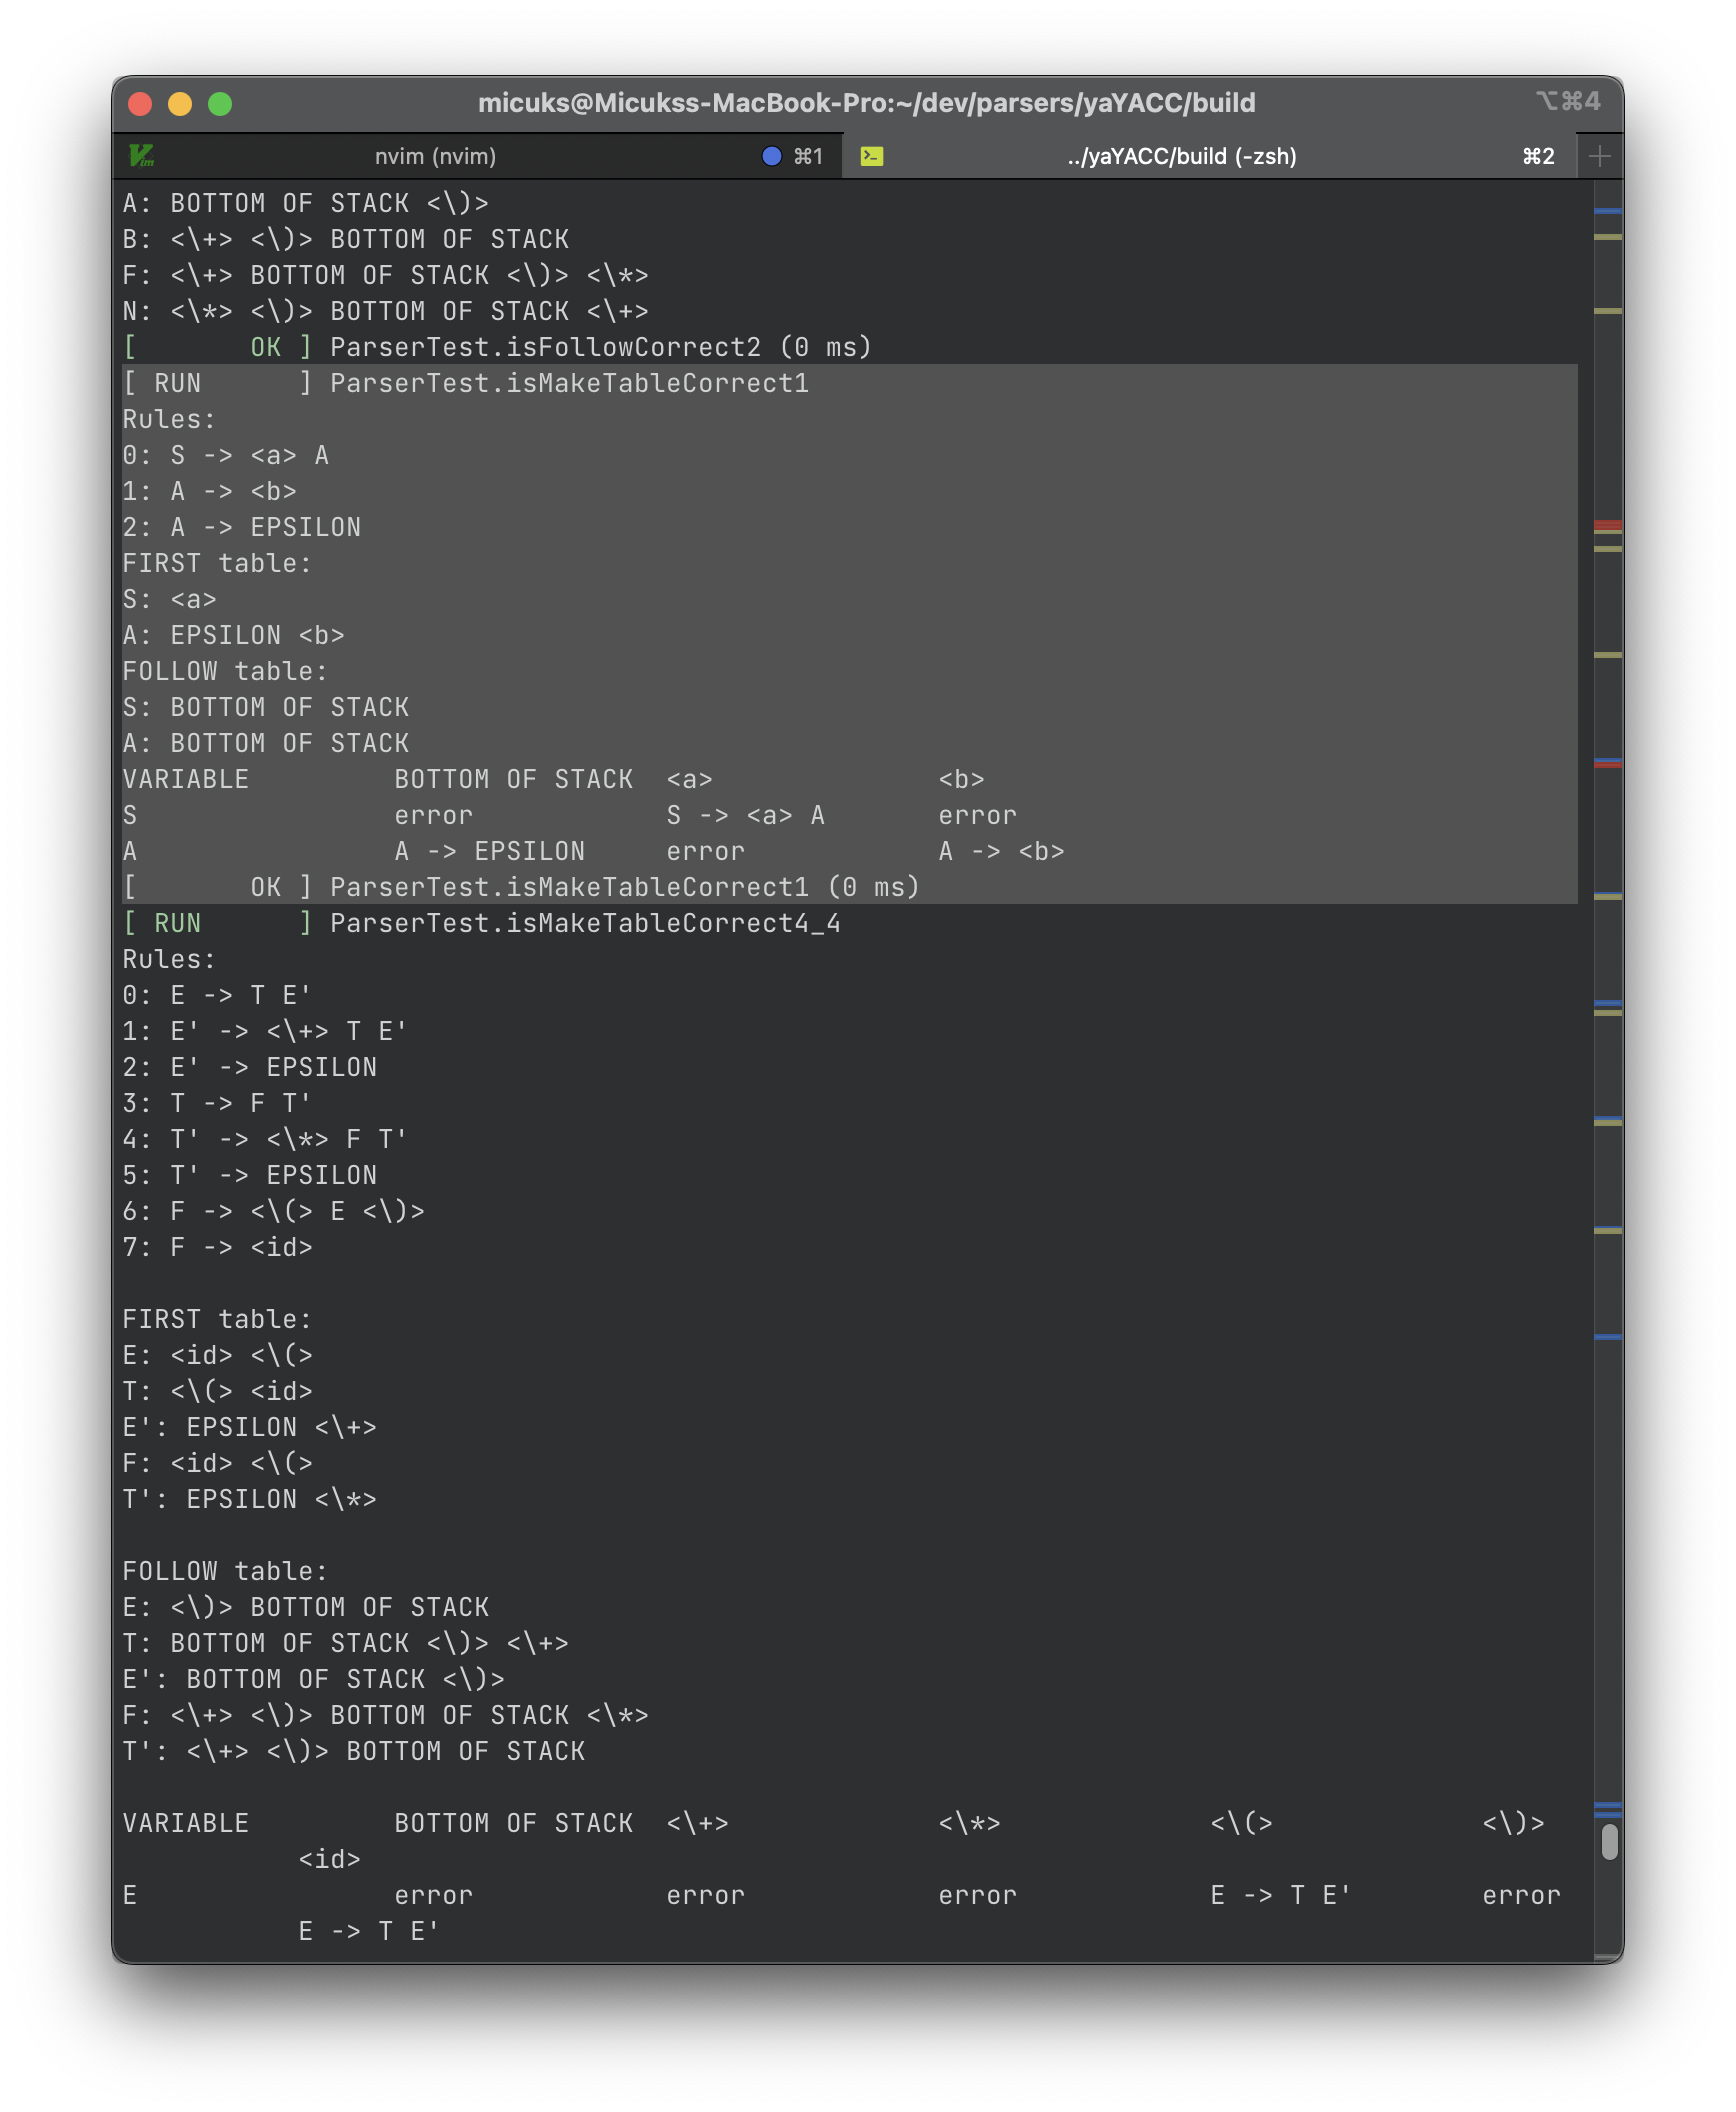
\includegraphics[width=0.95\textwidth]{figures/ll1分析表1.png}
	\end{center}
	\caption{简单文法的语法分析表}
	\label{fig:简单文法的语法分析表}
\end{figure}

较复杂的文法进行测试, 同样得到正确输出, 如图\ref{fig:复杂文法的语法分析表}.
\lstinputlisting[language=c++]{../grammars/g2.txt}

\begin{figure}[ht!]
	\begin{center}
		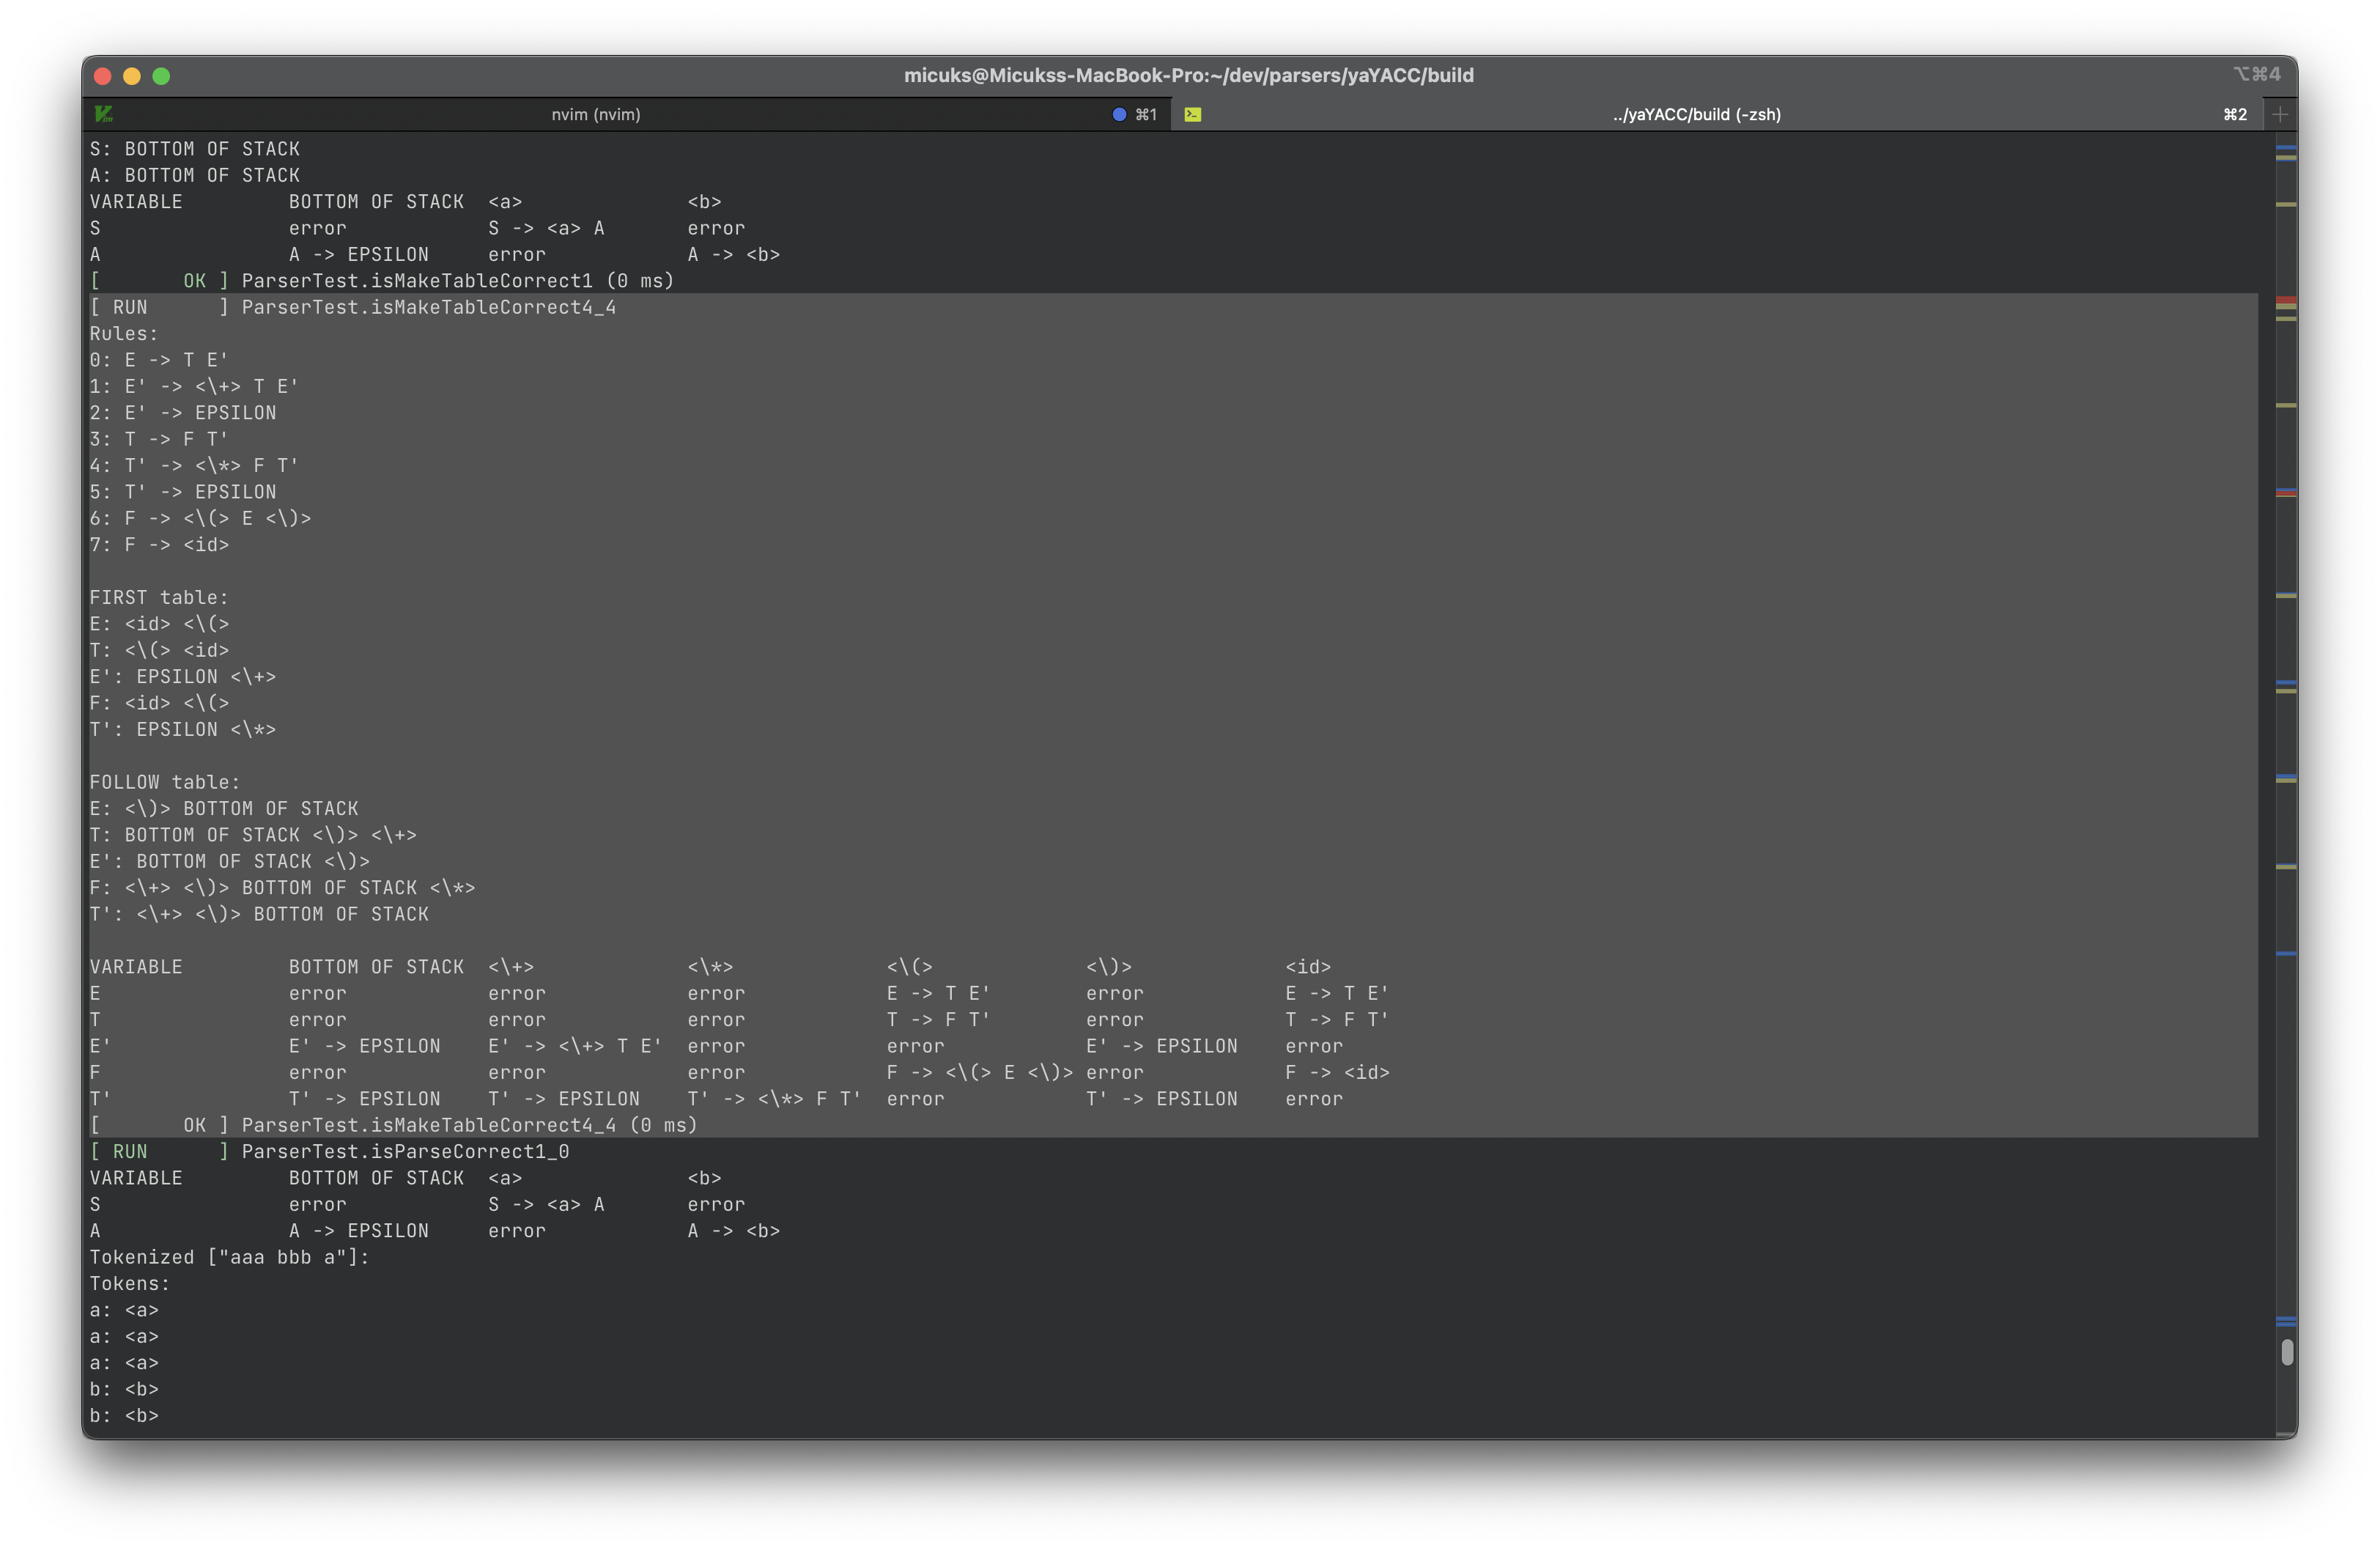
\includegraphics[width=0.95\textwidth]{figures/ll1分析表2.png}
	\end{center}
	\caption{复杂文法的语法分析表}
	\label{fig:复杂文法的语法分析表}
\end{figure}

使用简单文法生成的LL(1)分析表对字符串进行分析如图\ref{fig:简单文法的语法分析}. 两个字符串分别为"aaa bbb a", 和"   a
b   ", 其中, 第一个字符串会被拒绝, 第二个字符串会被接受,
关于程序结果是否正确的判断, 都是写在googletest中的检测内容, 具体可以见文末的代码清单.

\begin{figure}[ht!]
	\begin{center}
		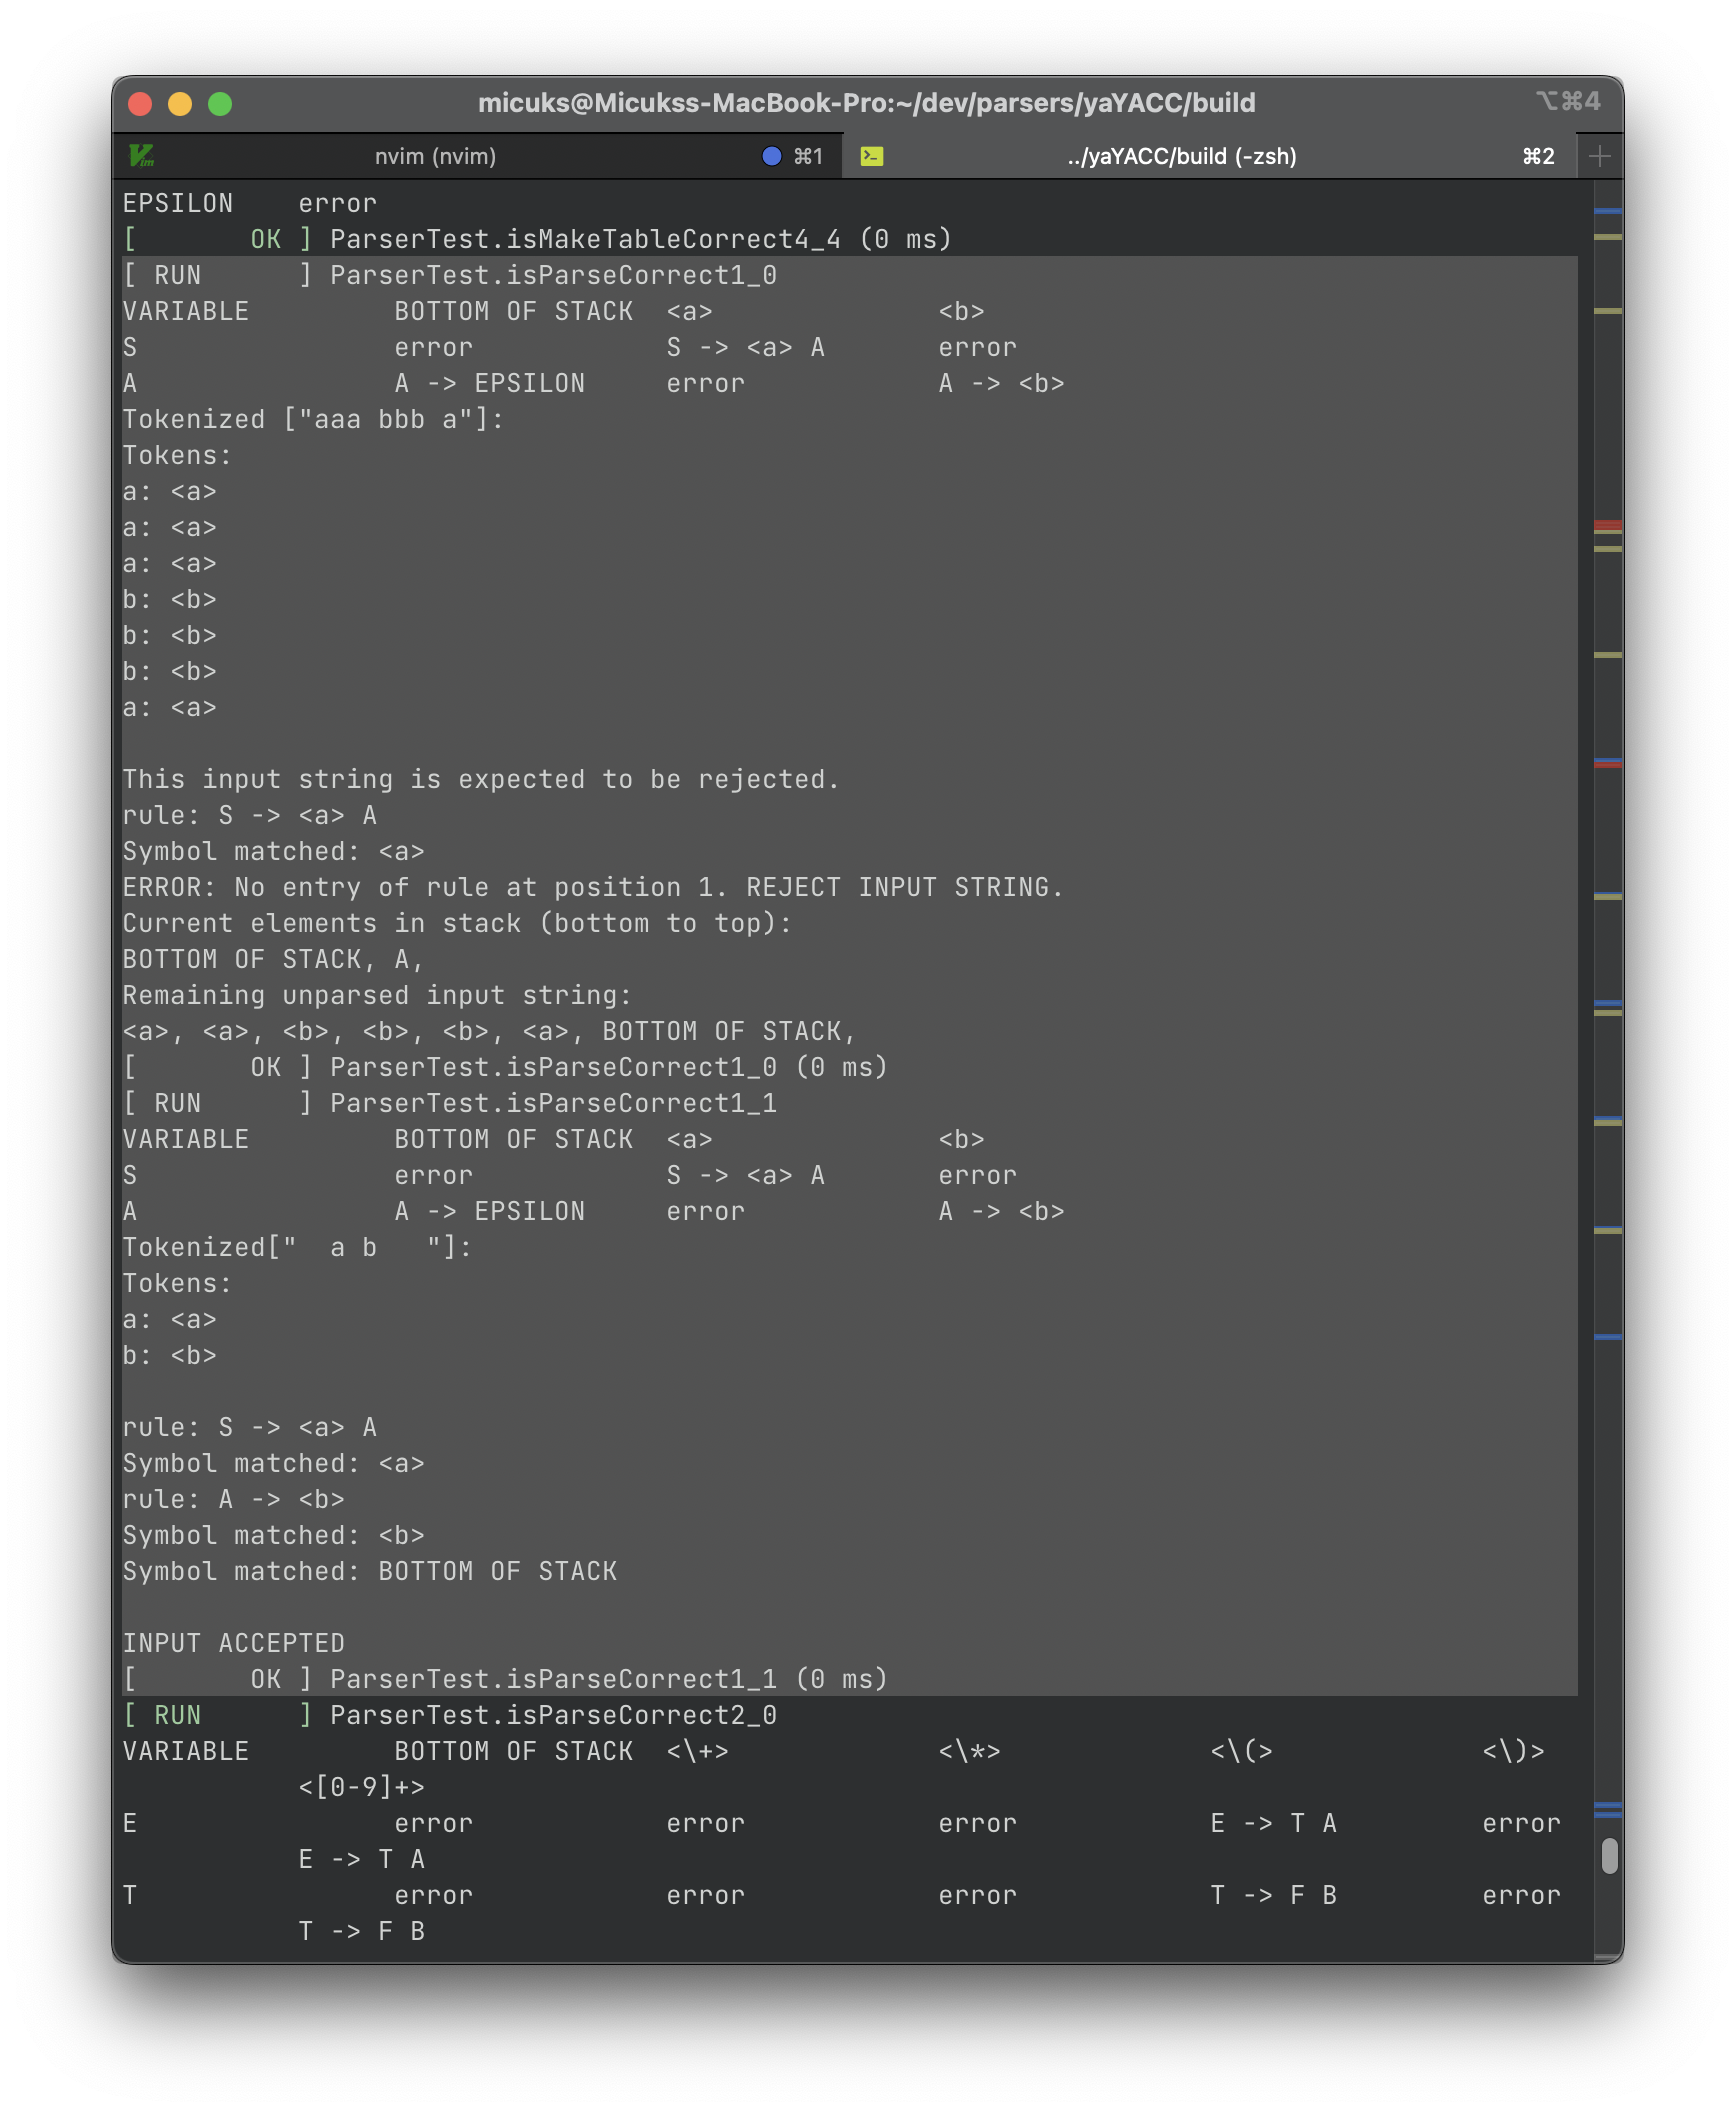
\includegraphics[width=0.95\textwidth]{figures/ll1分析输入1.png}
	\end{center}
	\caption{简单文法的语法分析}
	\label{fig:简单文法的语法分析}
\end{figure}

使用复杂文法进行分析同样得到正确结果, 如图\ref{fig:复杂文法的语法分析}.
输入串为"1+2+3+", 会被拒绝.

\begin{figure}[ht!]
	\begin{center}
		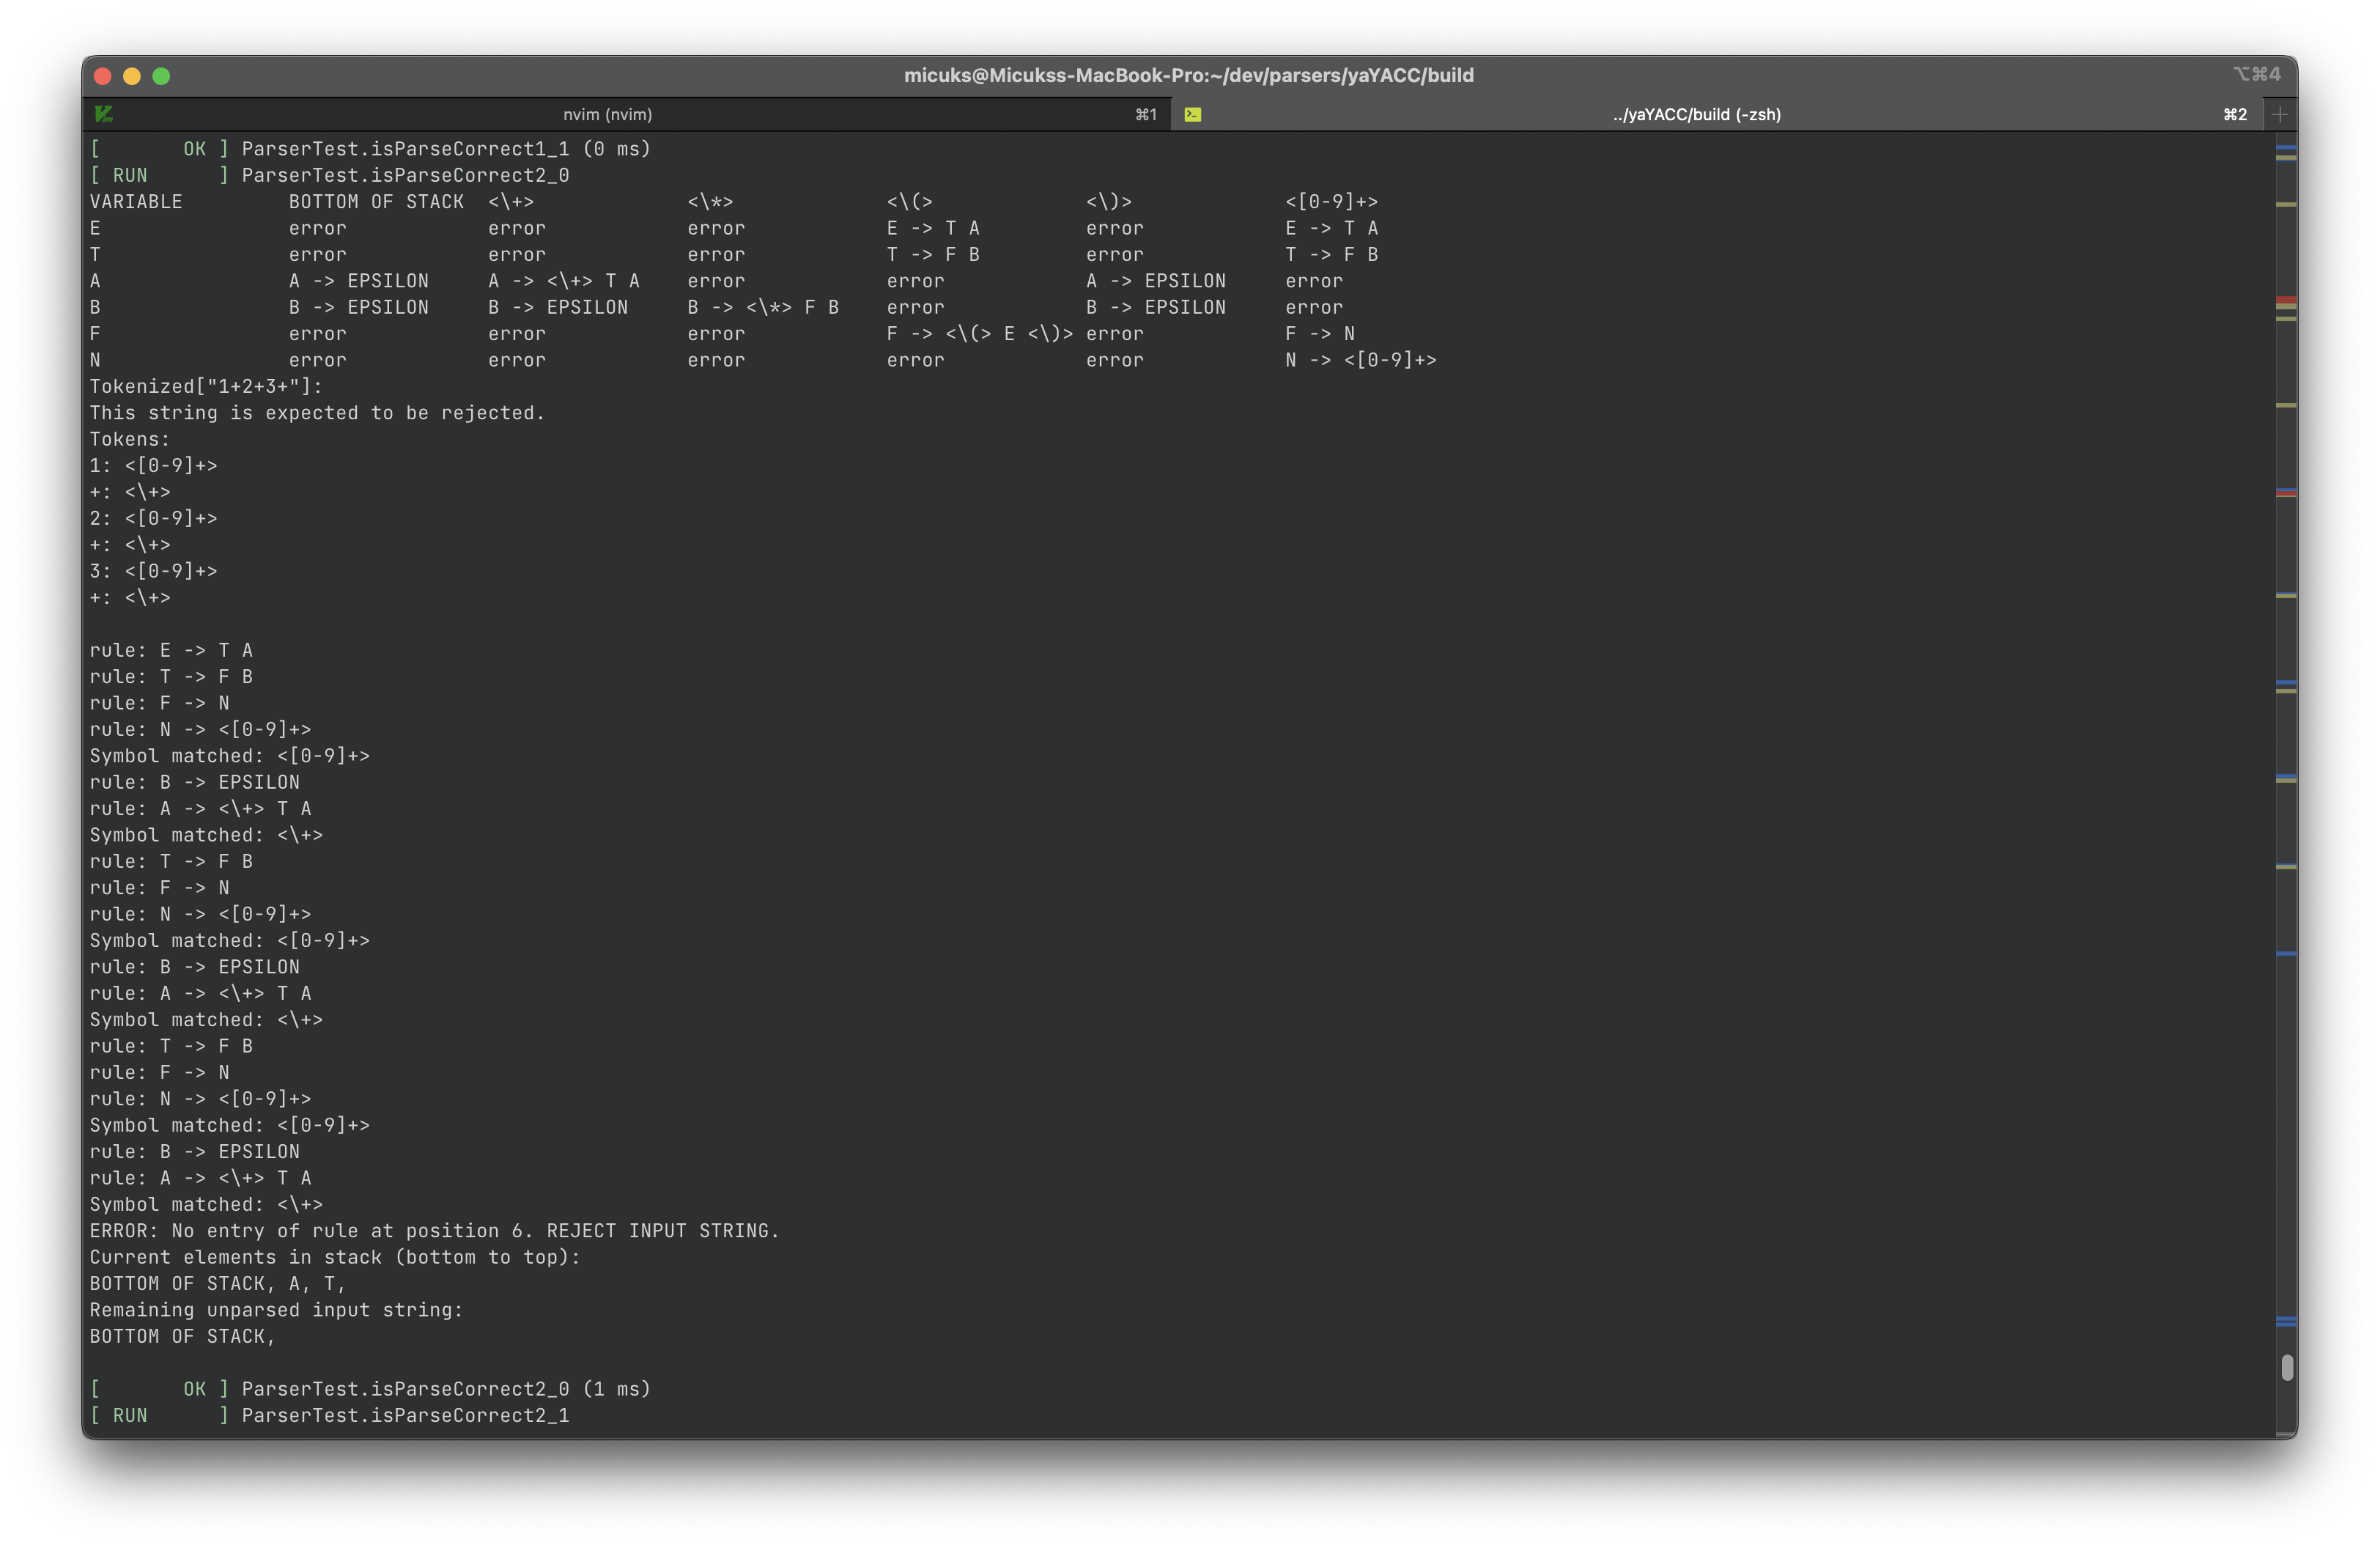
\includegraphics[width=0.95\textwidth]{figures/ll1分析输入20.png}
	\end{center}
	\caption{复杂文法的语法分析}
	\label{fig:复杂文法的语法分析}
\end{figure}

分析另一字符串"423*384*23", 将被接受, 如图\ref{fig:复杂文法的语法分析2}.

\begin{figure}[ht!]
	\begin{center}
		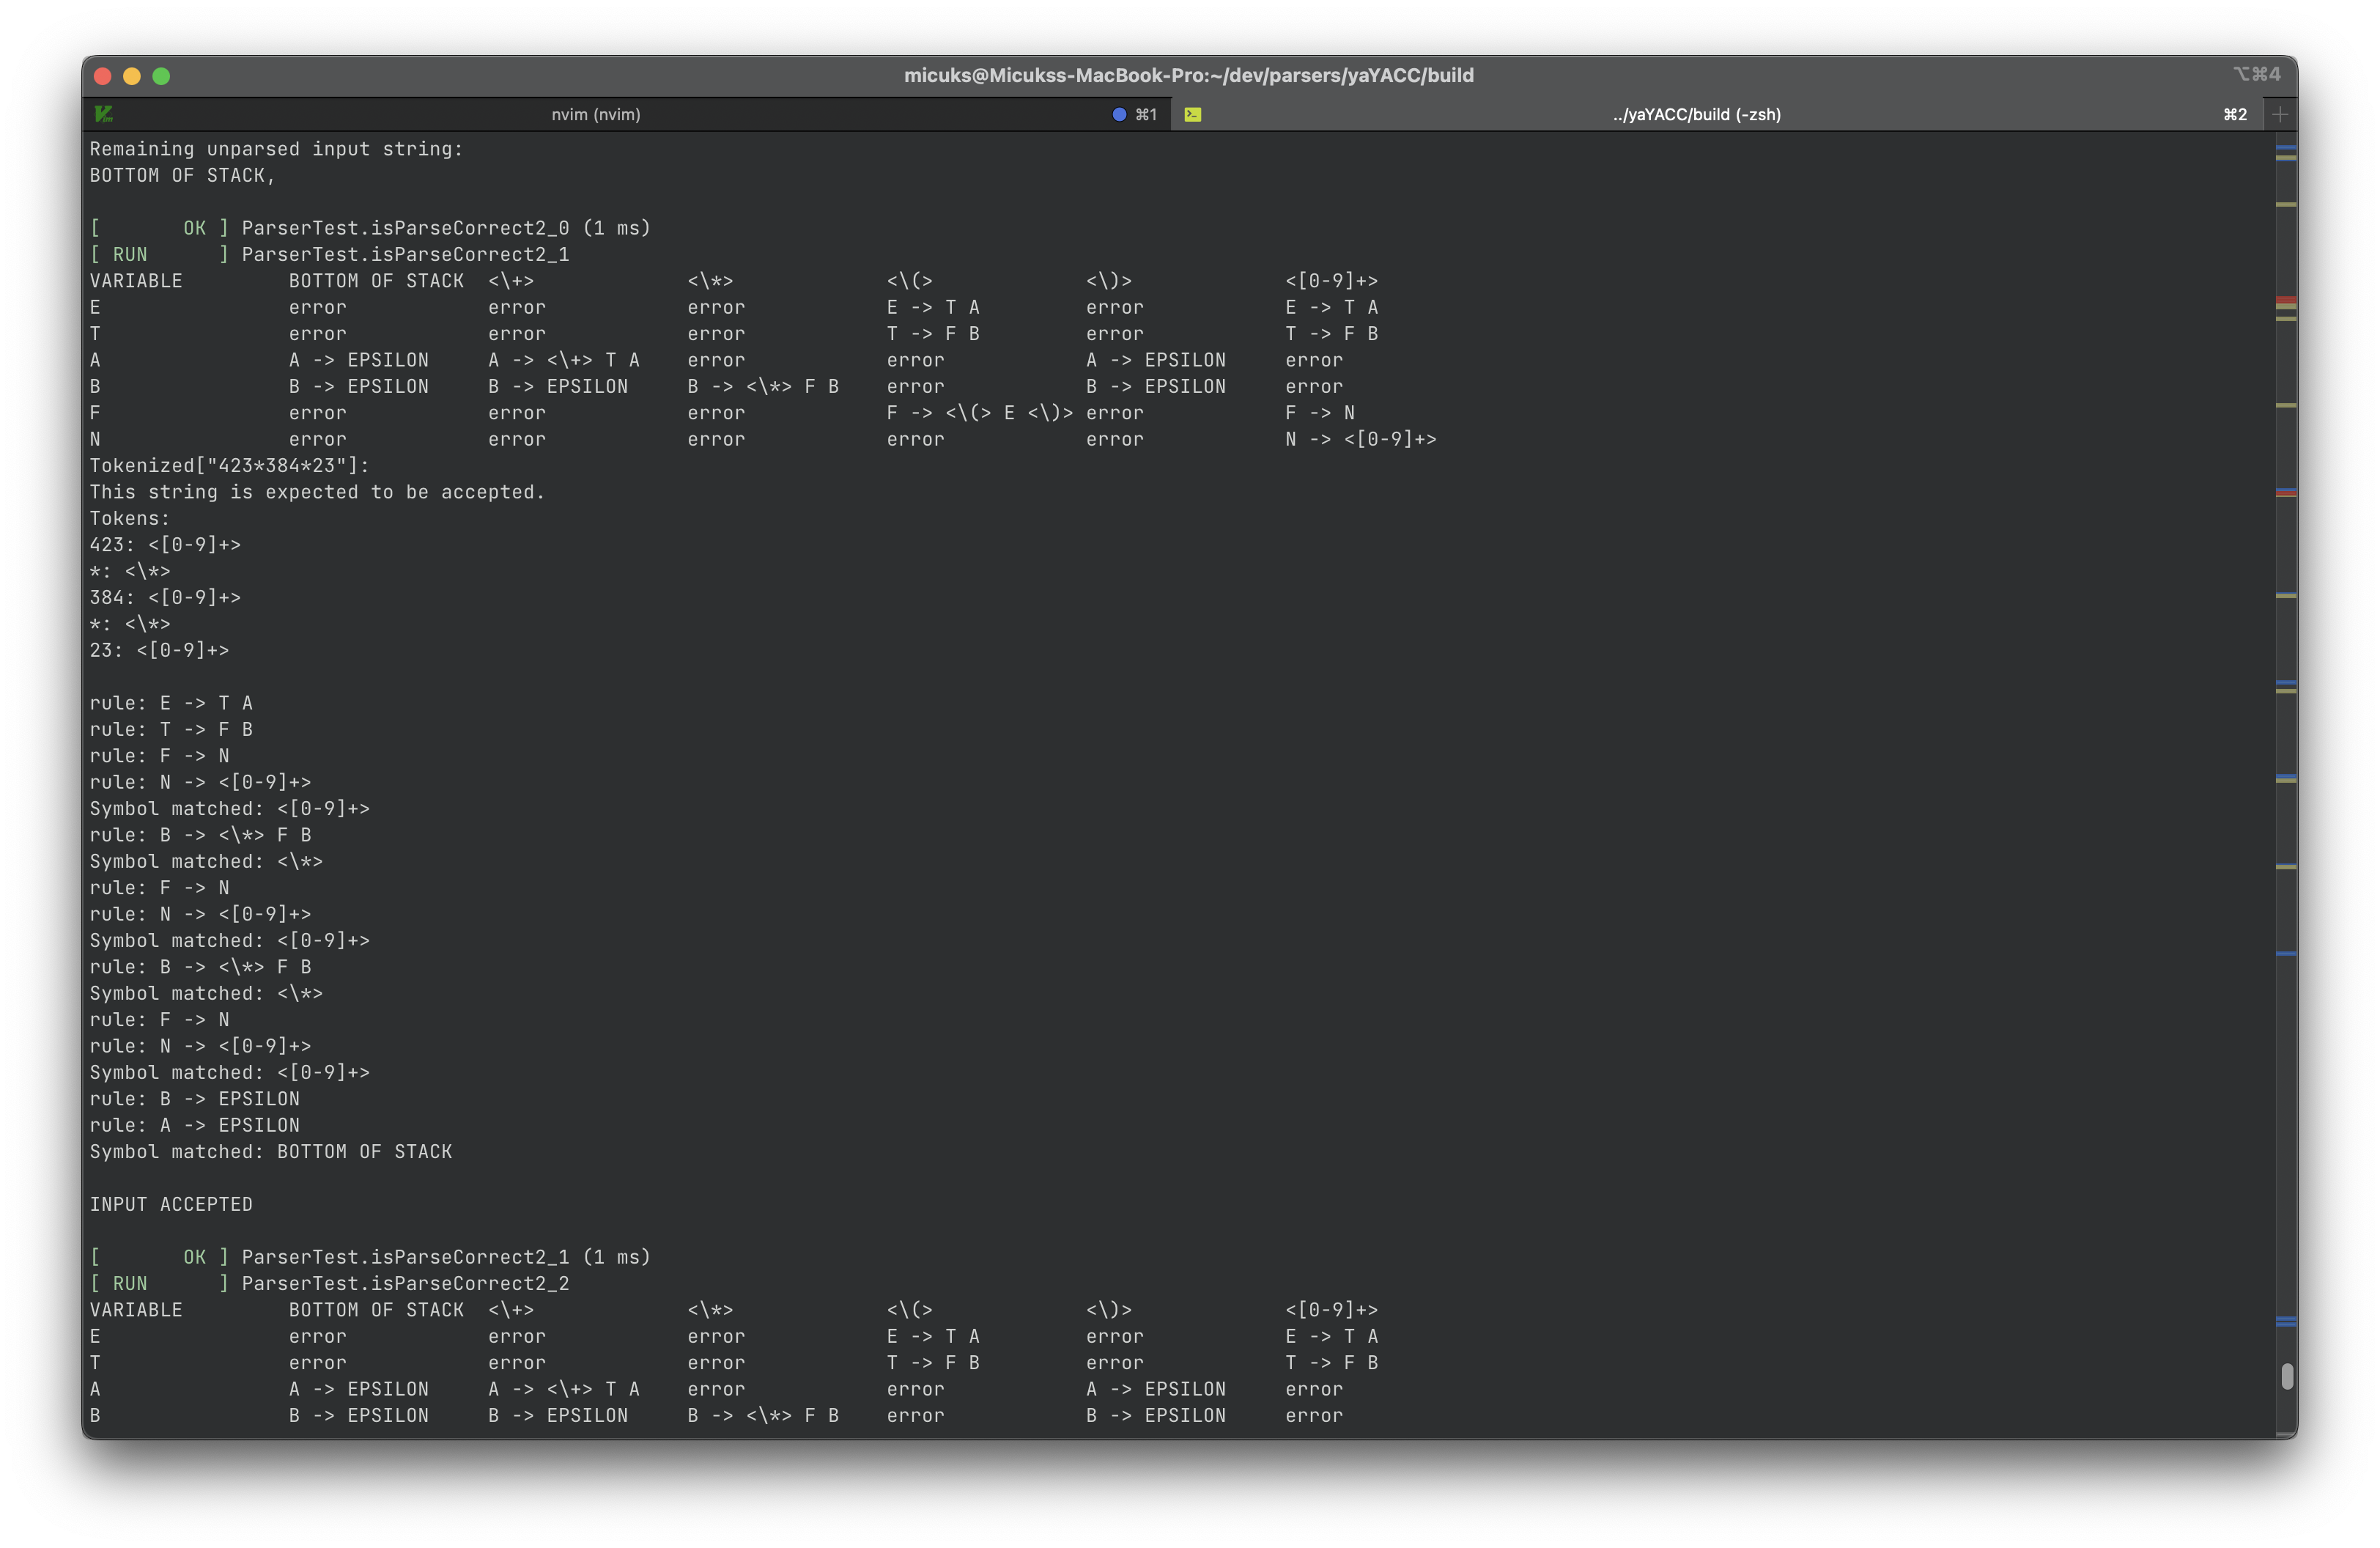
\includegraphics[width=0.95\textwidth]{figures/ll1分析输入21.png}
	\end{center}
	\caption{复杂文法的语法分析}
	\label{fig:复杂文法的语法分析2}
\end{figure}

\subsection{消除左递归测试}
使用作业所给文法作为输入进行测试:
\lstinputlisting[language=c++]{../grammars/g3.txt}

使用多个不同的字符串和文法对LL(1)语法分析程序进行充分测试, 在此不一一展示,
运行日志均放在文末附录.

\subsection{LR(1)语法分析程序}
\subsubsection{生成规范族DFA和LR(1)分析表测试}

首先使用简单的文法进行测试, 文法如下:
\lstinputlisting[language=c++]{../grammars/g1.txt}

测试得到的项目集DFA如图\ref{fig:简单文法的LR1分析测试}LR1 Item Sets部分,
LR(1)分析表如LR1 Parse Table部分,
对输入字符串"  a  b  "进行分析得到的结果紧接在LR1分析表下面, 分析结果为接受.
分析结果氛围三栏, 第一栏为栈, 状态栈和符号栈交叉存储; 第二栏为待分析的tokens,
其中BOTTOM OF STACK为栈底符号, 每个终结符被方括号<>括起; 最后一栏为Action,
表示此时进行的动作, 包括Shift, Reduce, Goto和ACCEPT, 以及出错信息.

\begin{figure}[ht!]
	\begin{center}
		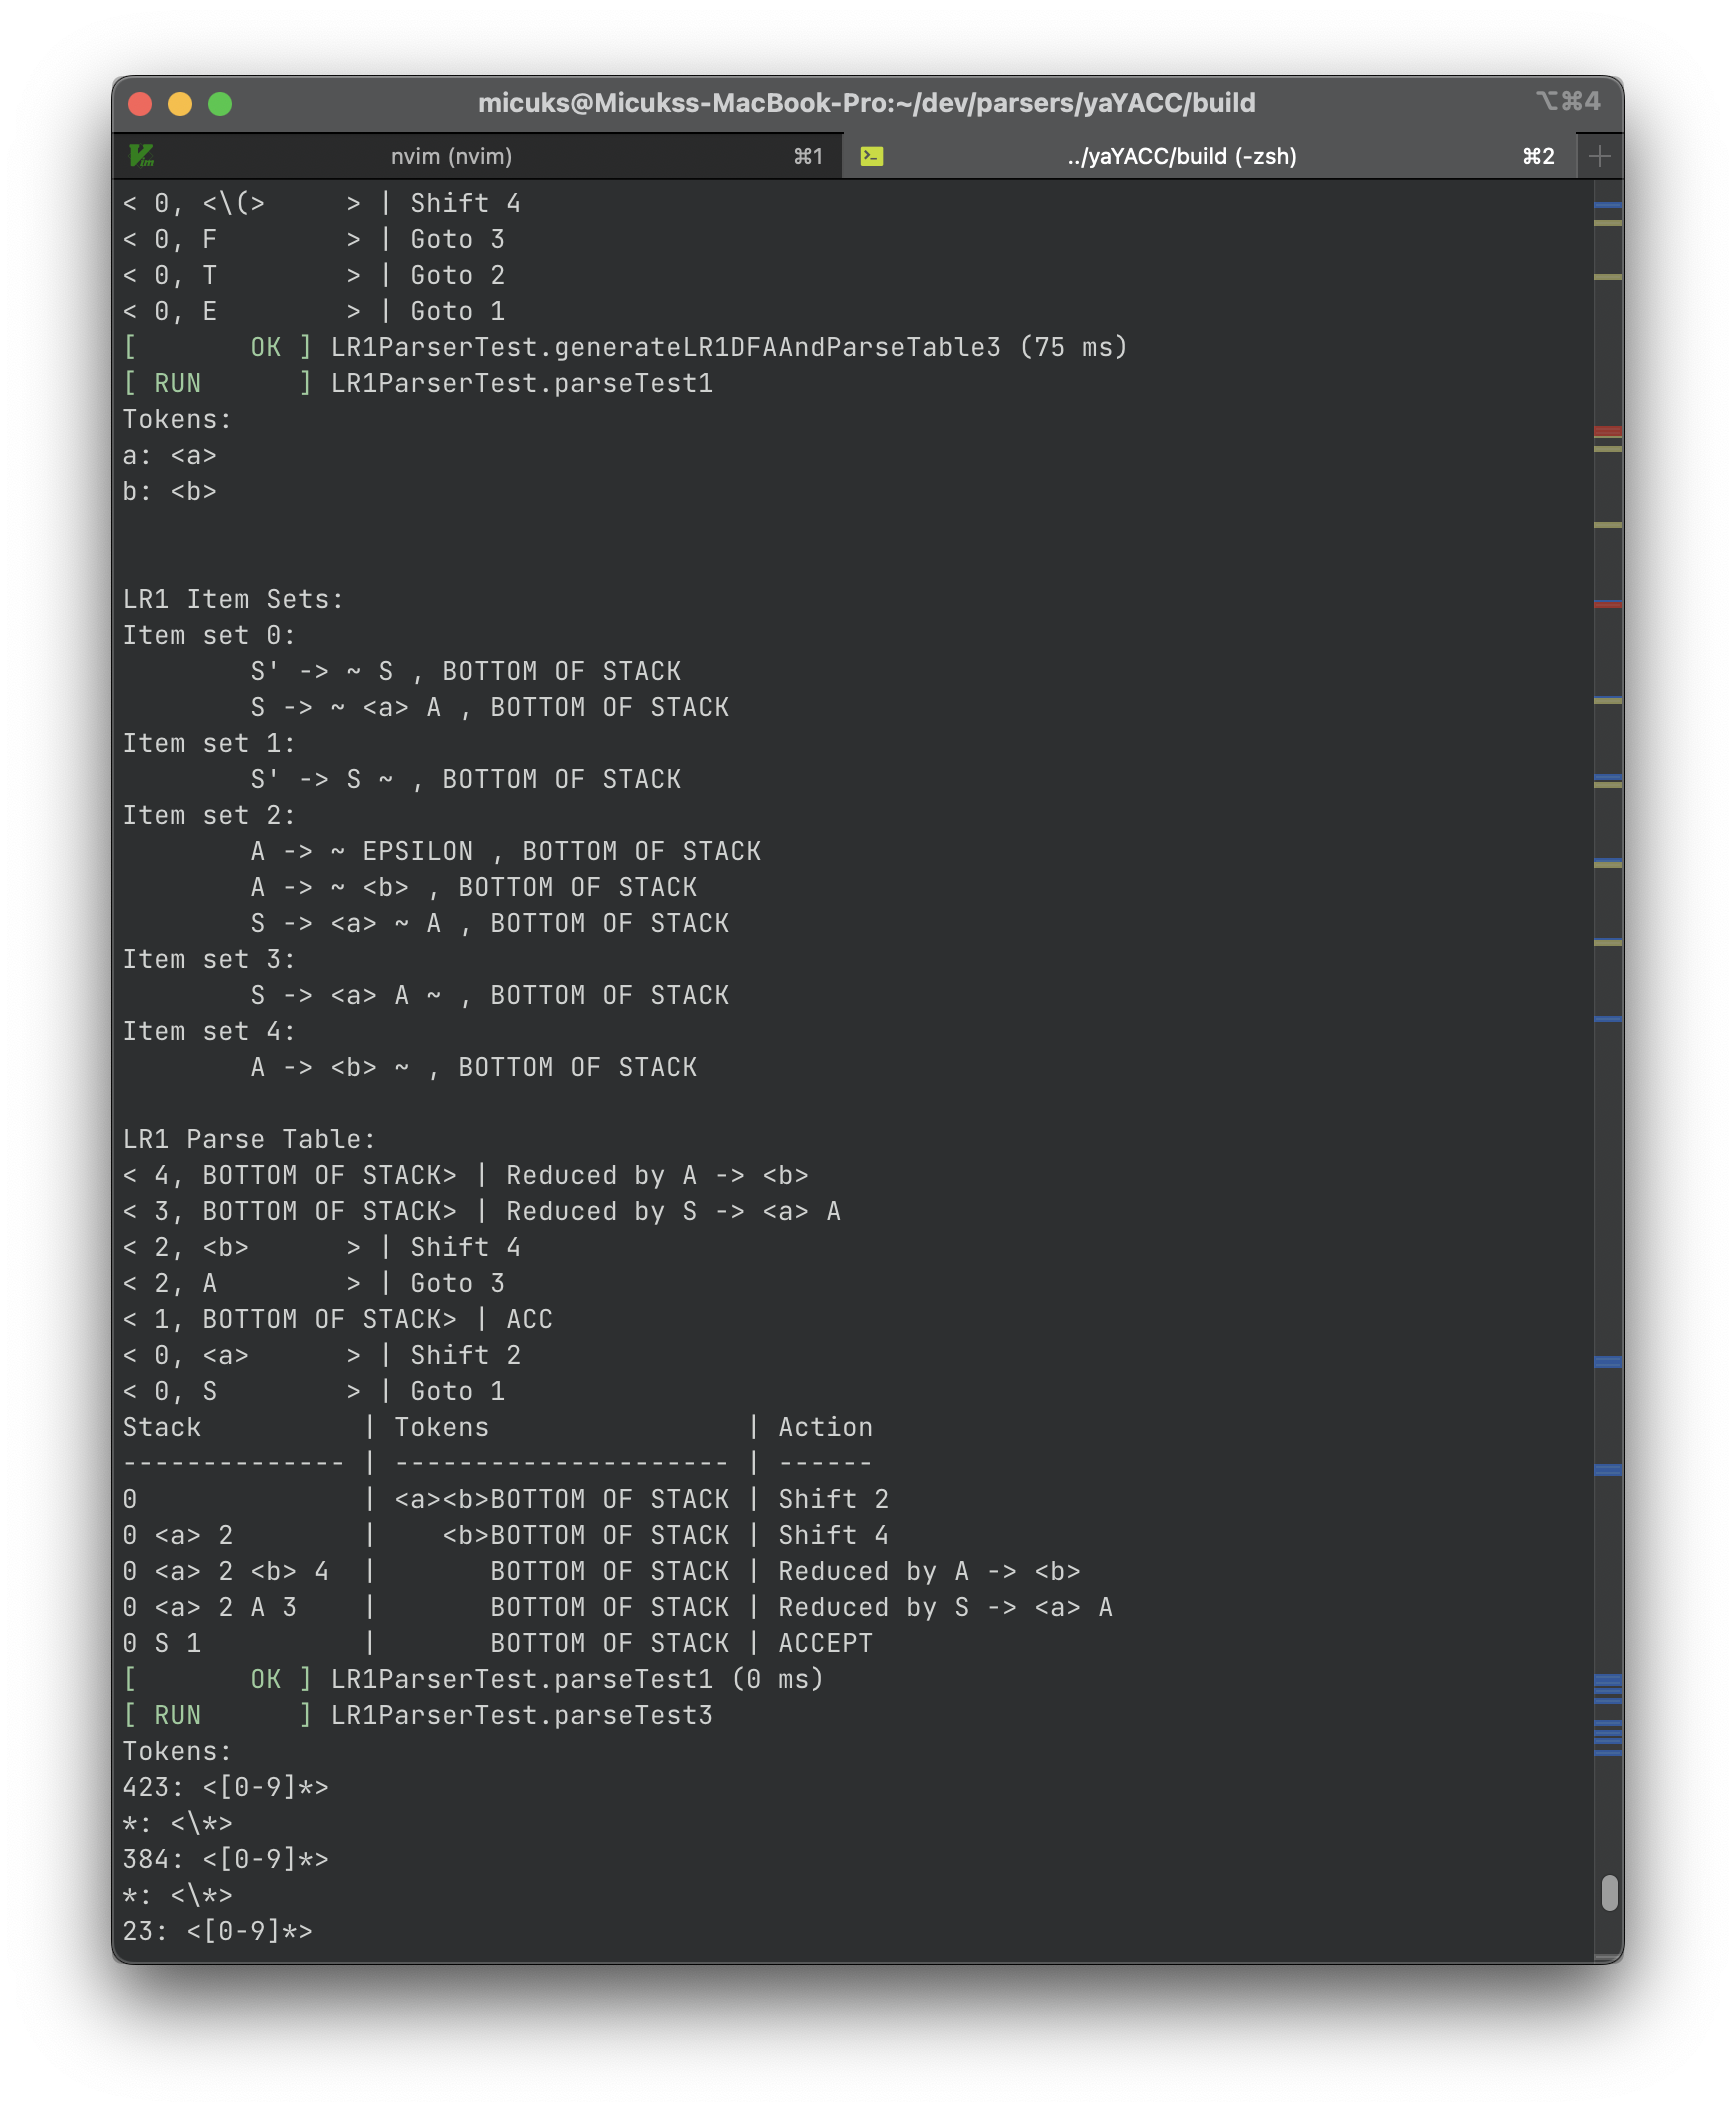
\includegraphics[width=0.95\textwidth]{figures/lr1分析1.png}
	\end{center}
	\caption{简单文法的LR1分析测试}
	\label{fig:简单文法的LR1分析测试}
\end{figure}

然后使用作业所给文法进行测试, 文法如下:
\lstinputlisting[language=c++]{../grammars/g3.txt}

其生成的项目集规范族DFA如下图\ref{fig:复杂文法的LR1项目集规范族DFA}.

\begin{figure}[ht!]
	\begin{center}
		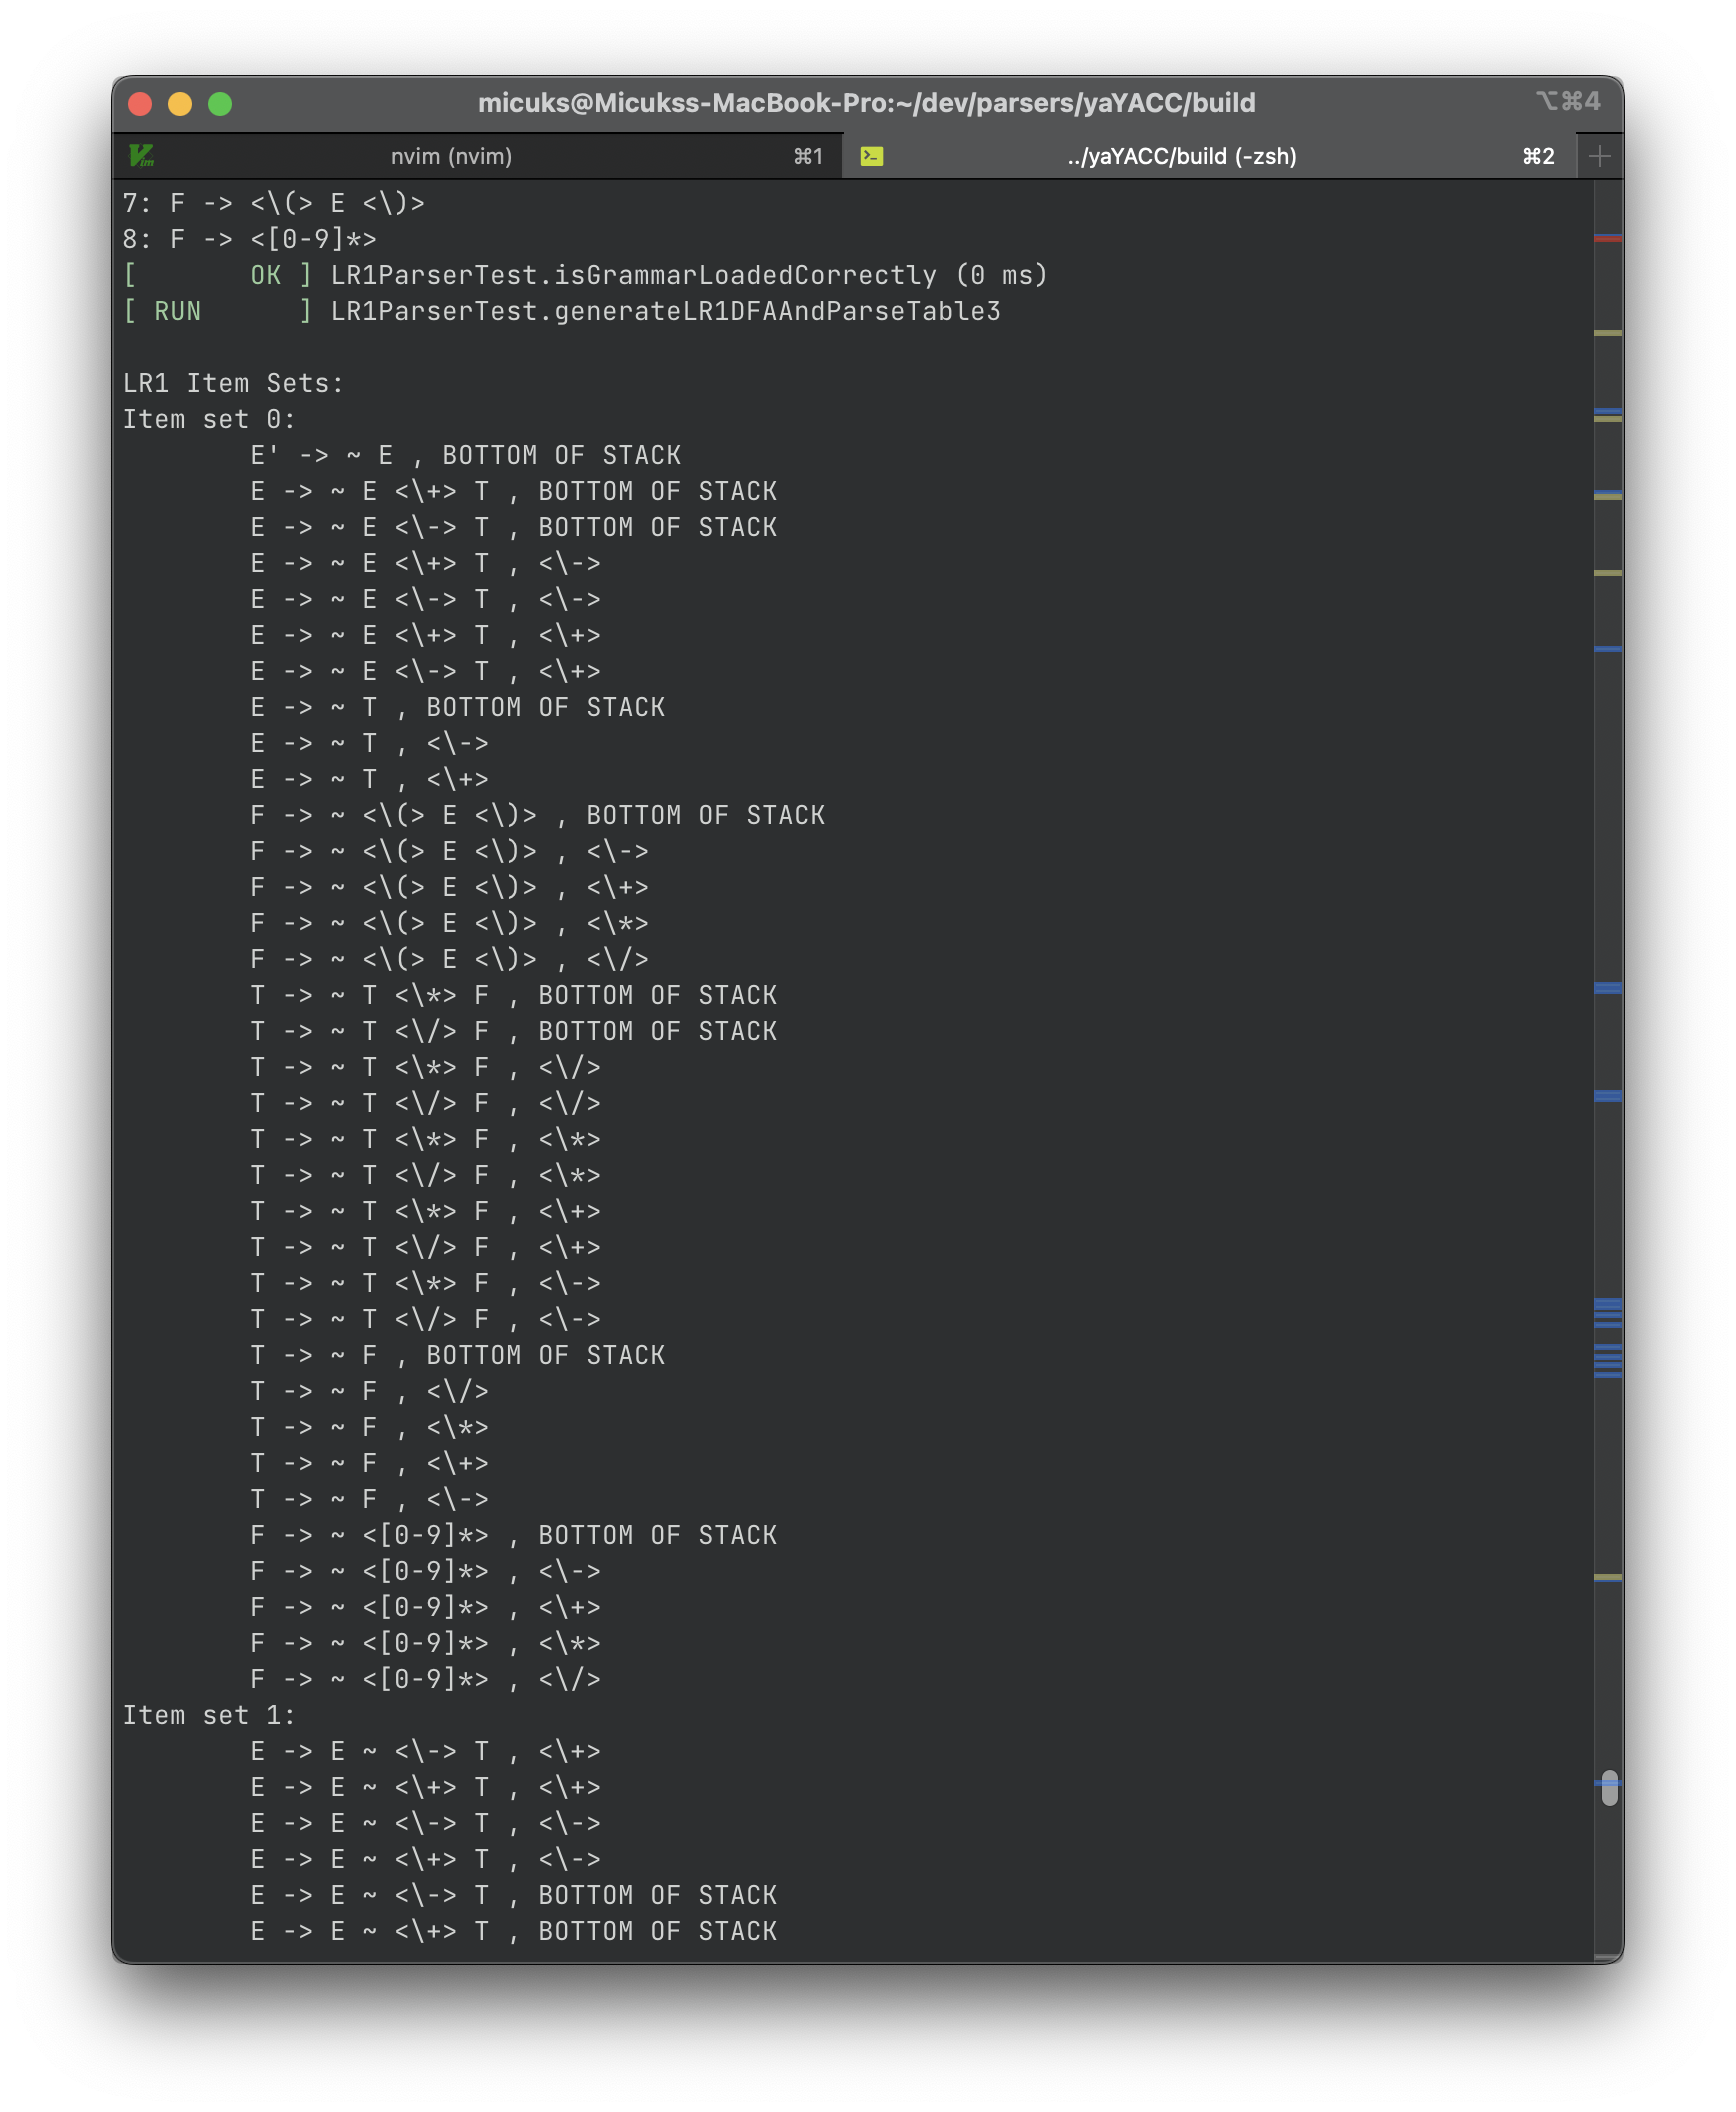
\includegraphics[width=0.95\textwidth]{figures/lr1规范族1.png}
	\end{center}
	\caption{复杂文法的LR1项目集规范族DFA}
	\label{fig:复杂文法的LR1项目集规范族DFA}
\end{figure}

生成的LR1分析表如下图\ref{fig:复杂文法的LR1分析表}:

\begin{figure}[ht!]
	\begin{center}
		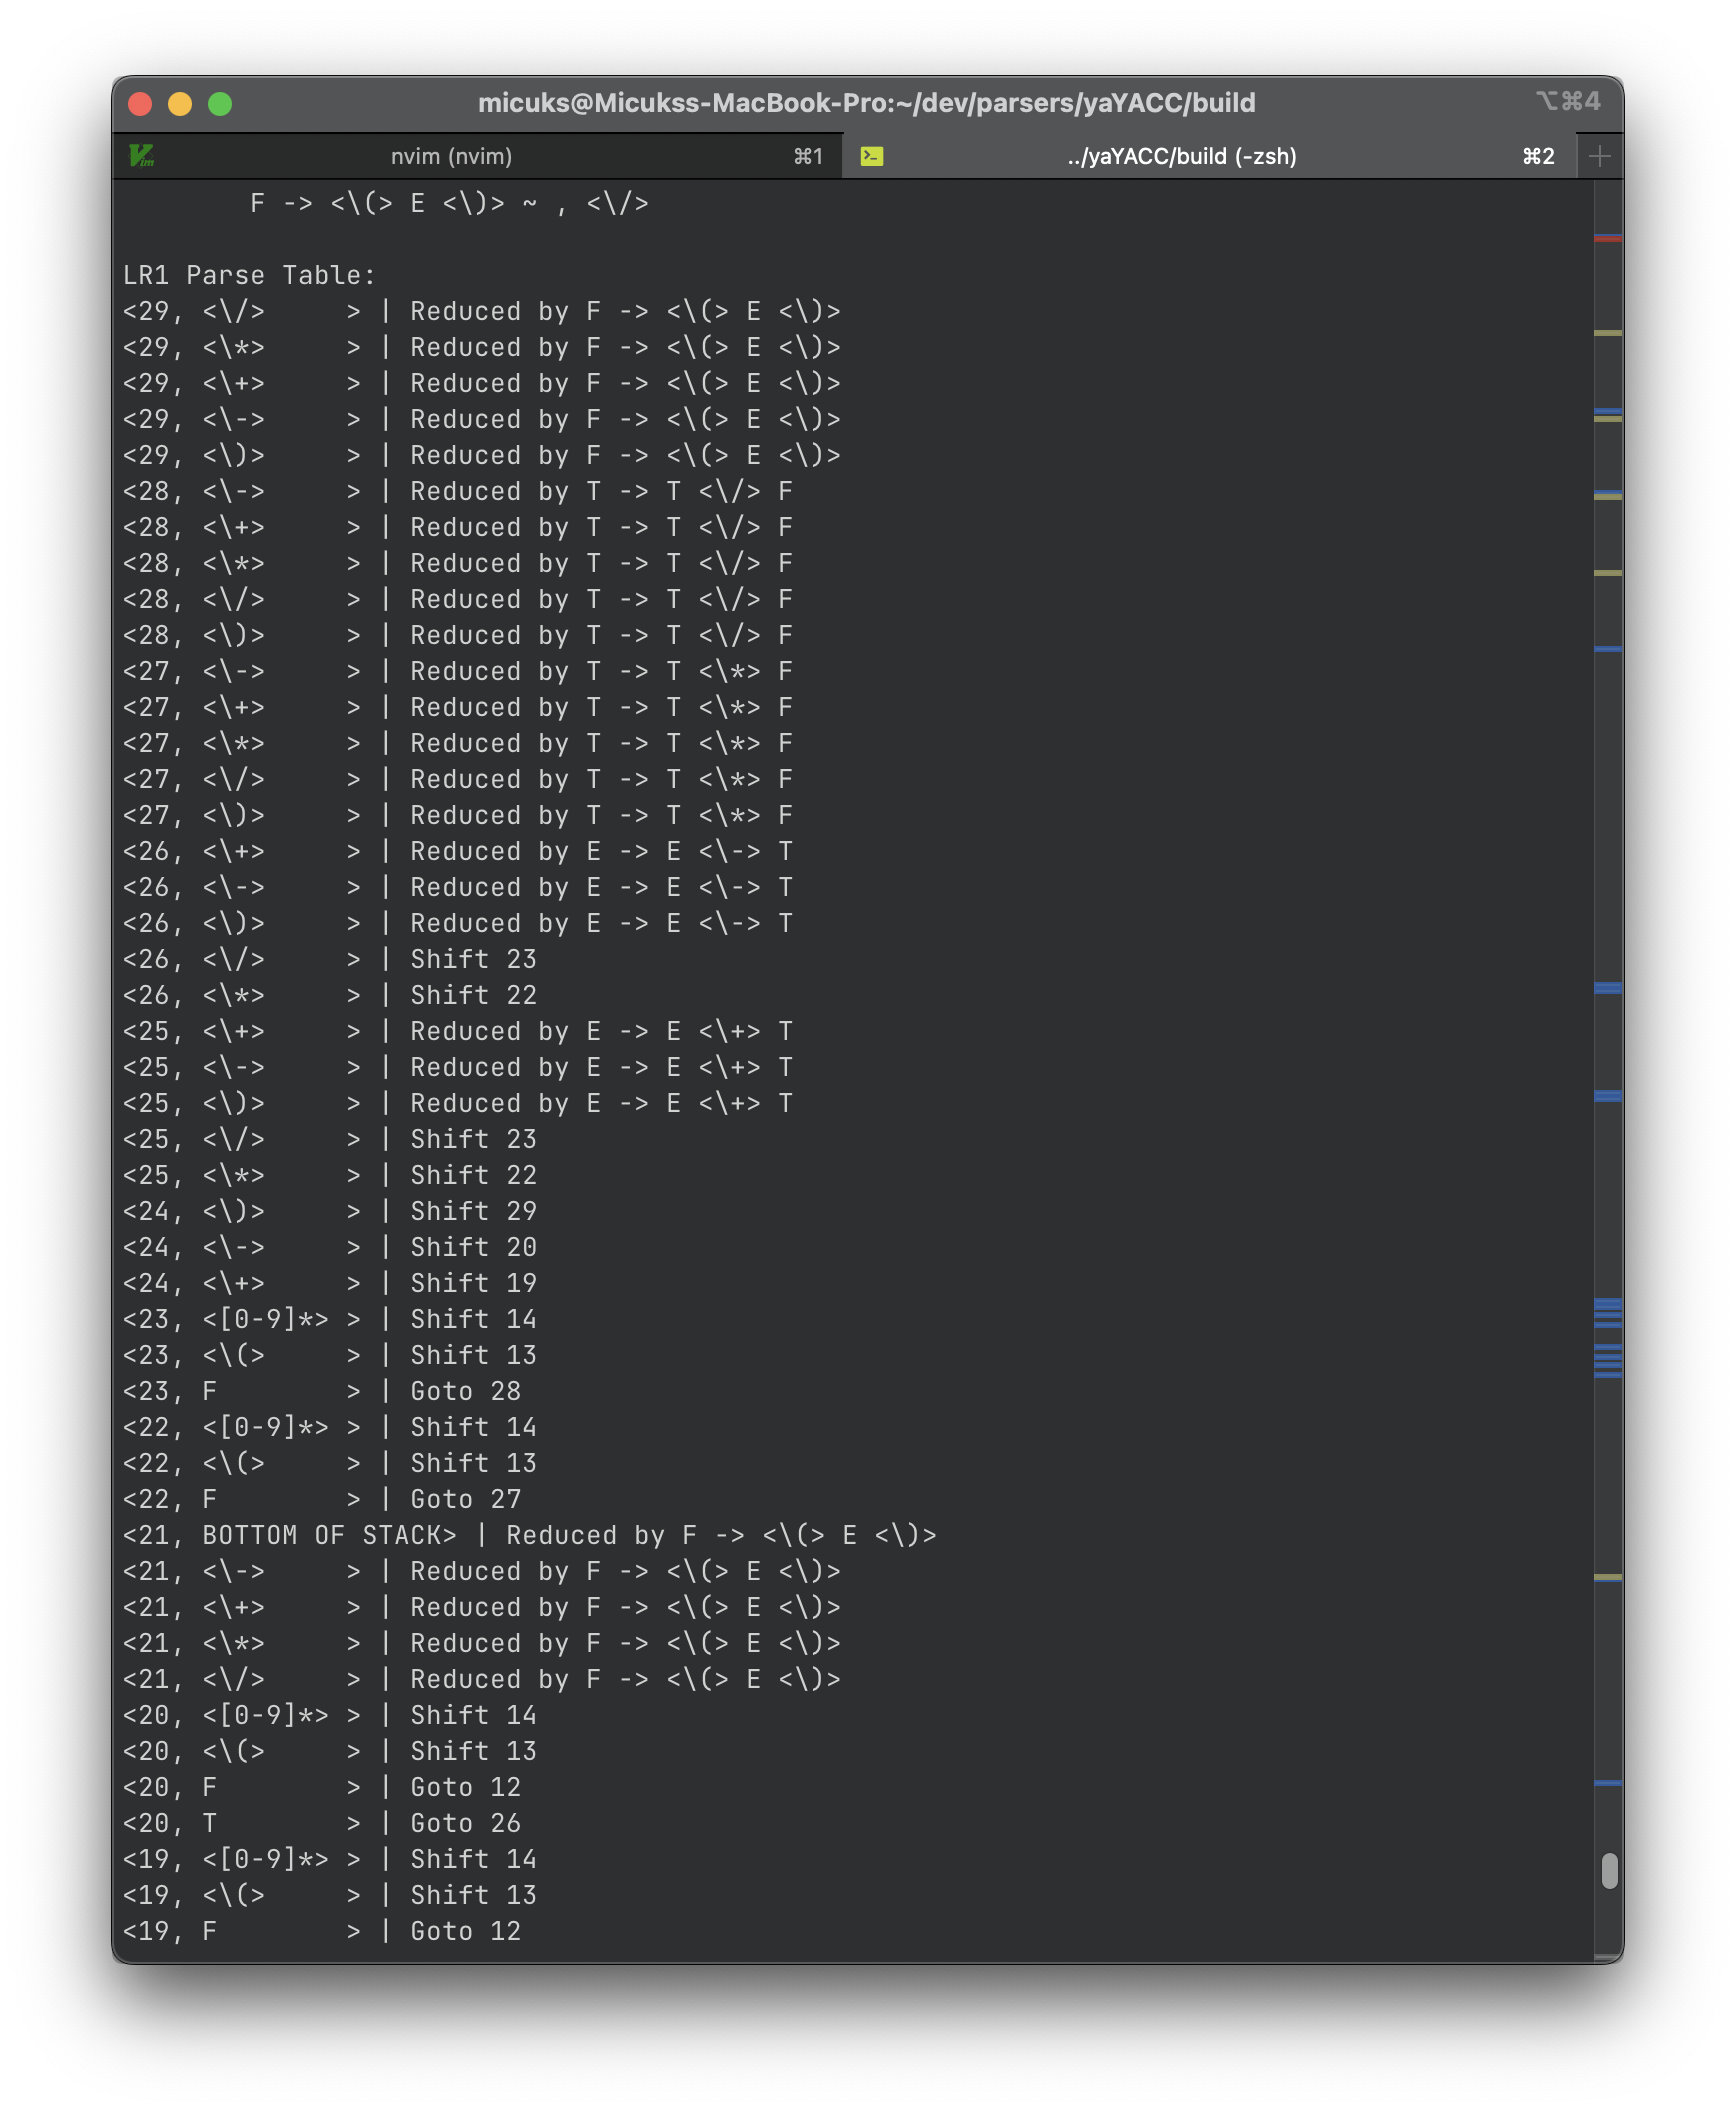
\includegraphics[width=0.95\textwidth]{figures/lr1复杂分析表1.png}
	\end{center}
	\caption{复杂文法的LR1分析表}
	\label{fig:复杂文法的LR1分析表}
\end{figure}

由于DFA有30个状态, 输出太长, 所以完整输出放在了附录中.

\subsubsection{对输入字符串进行分析测试}

使用作业所给文法, 对简单的输入字符串"423*384*23"进行测试, 结果为接受,
测试方式与上面简单文法相同, 输出如图.
\begin{figure}[ht!]
	\begin{center}
		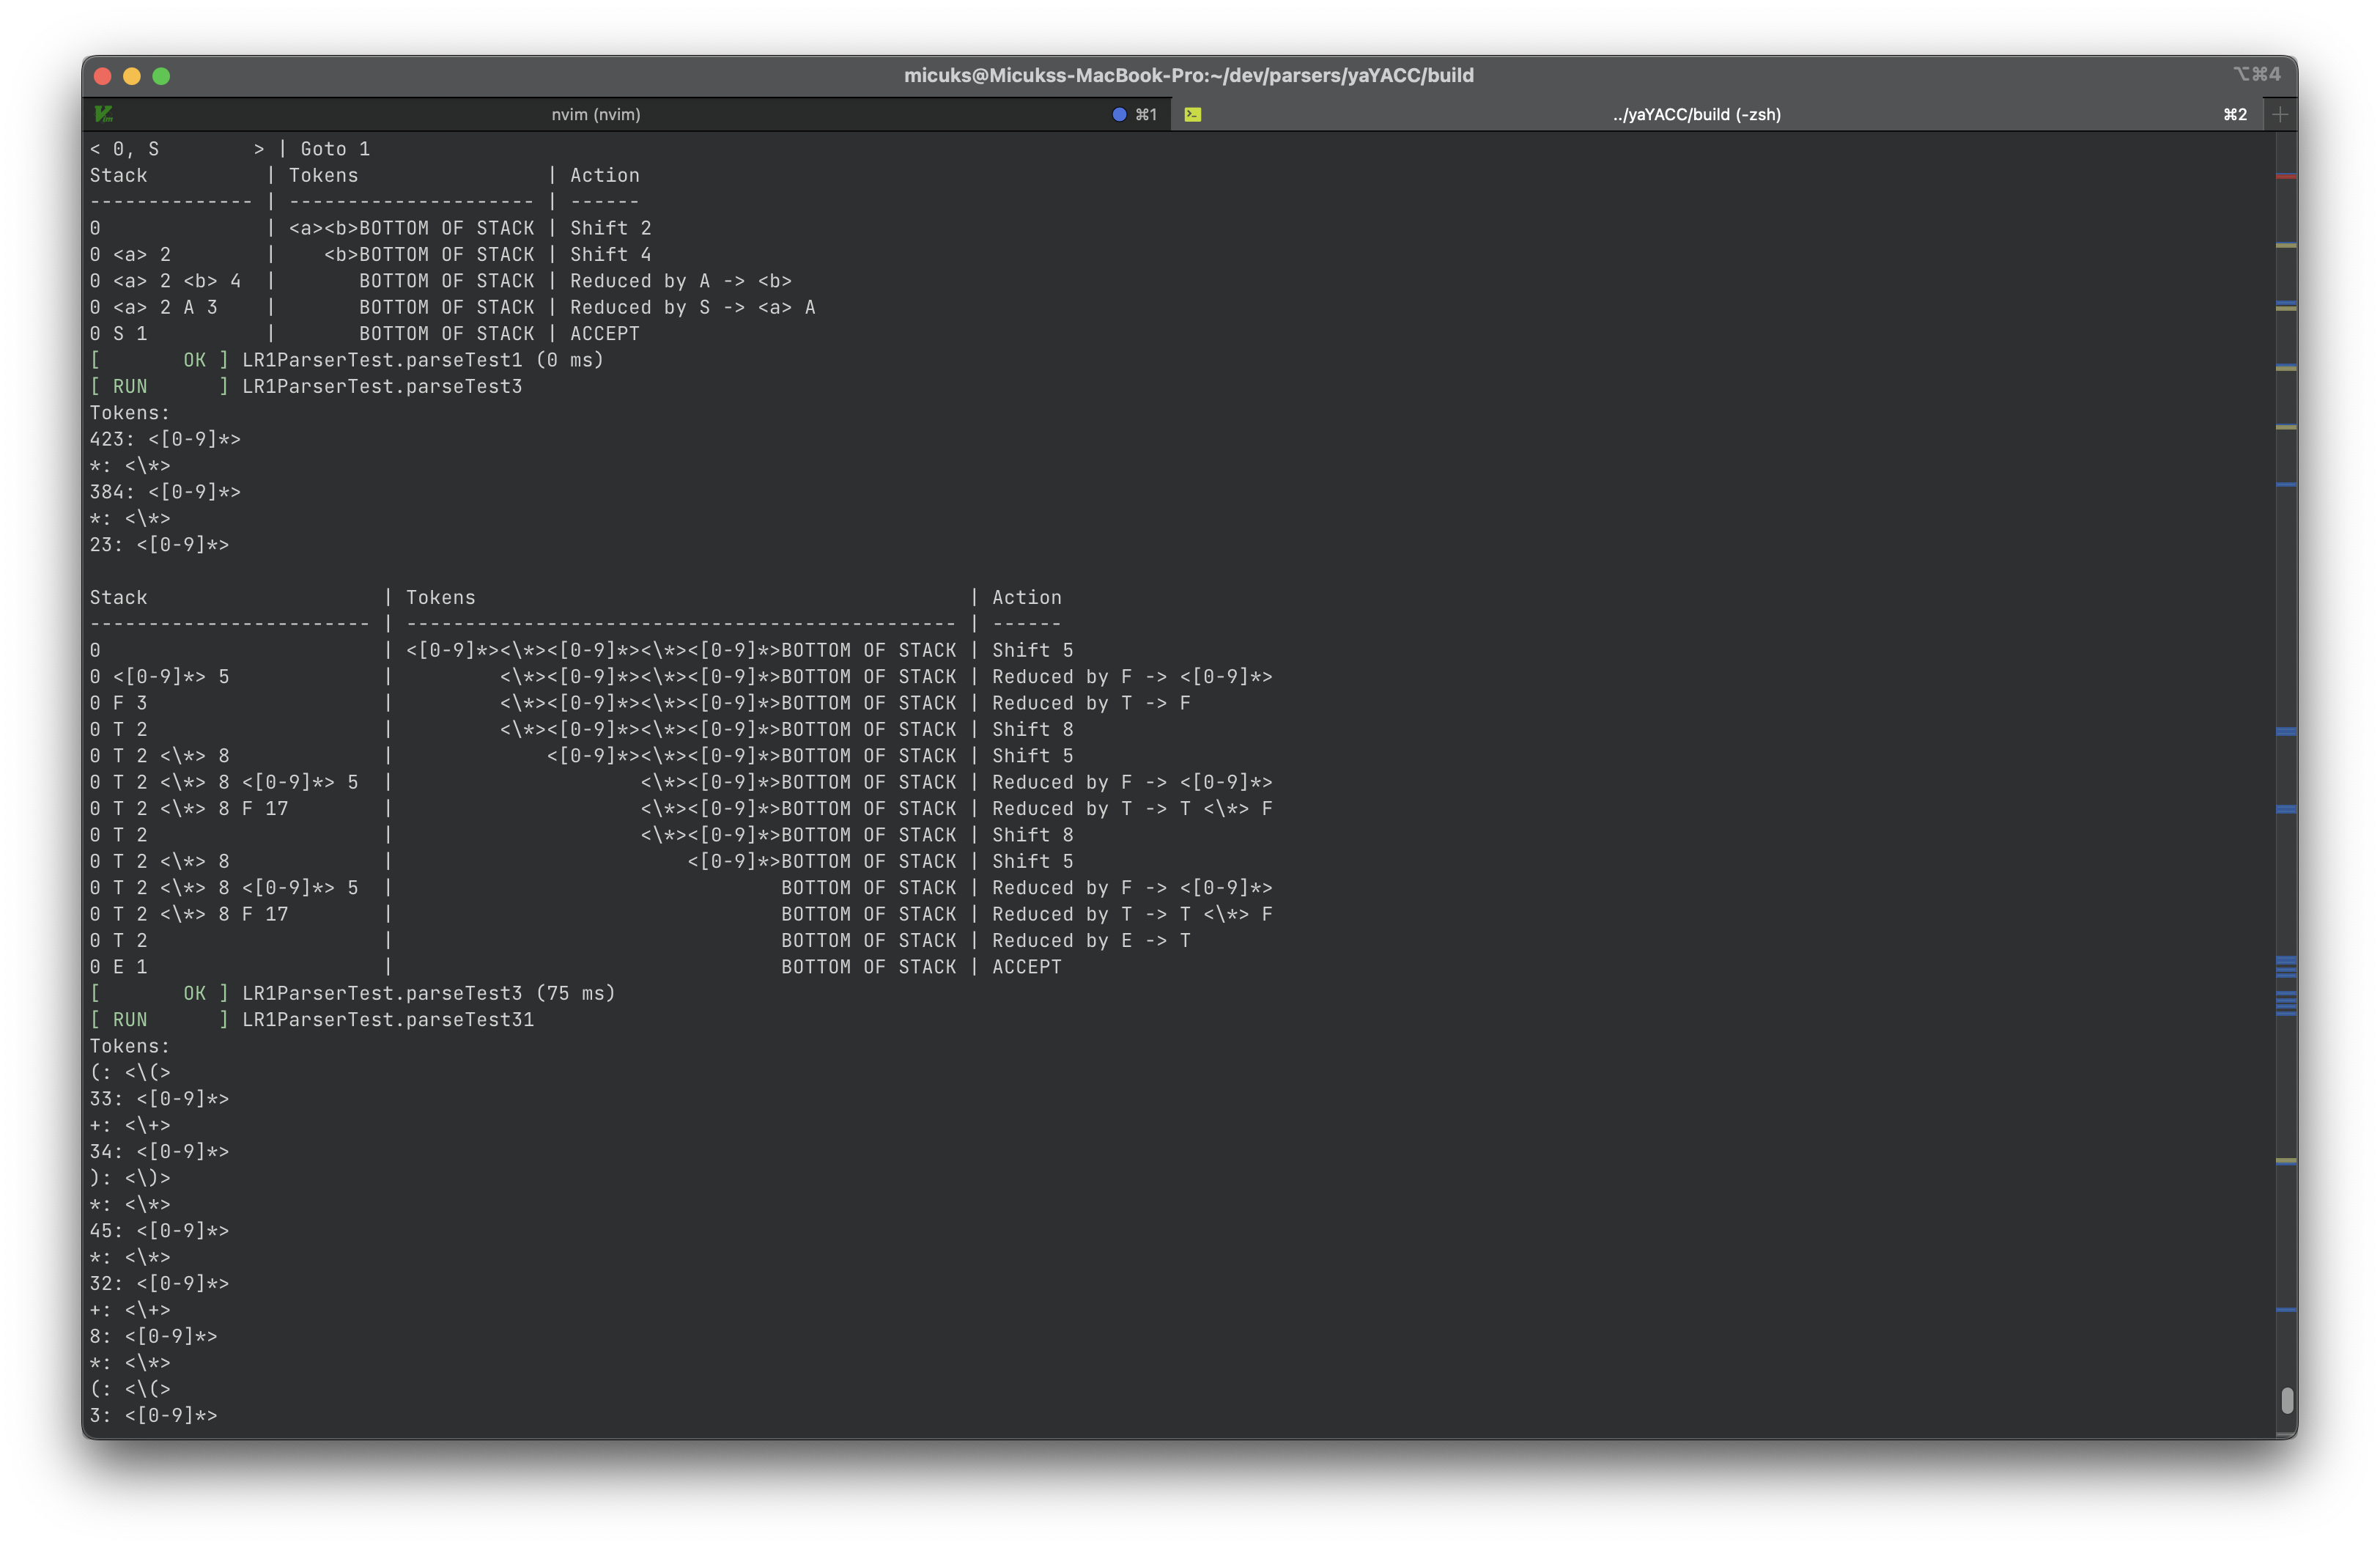
\includegraphics[width=0.95\textwidth]{figures/lr1复杂分析1.png}
	\end{center}
	\caption{复杂文法的LR1分析1}
	\label{fig:复杂文法的LR1分析1}
\end{figure}

对较复杂的输入串"(33+34)*(45*32)+8*(3*1+3)"进行分析, 结果为接受,
如图\ref{fig:复杂文法的LR1分析2}.
由于输入的文法中对数字均使用了相同的正则表达式表示, 所以Tokens看起来不清晰.
可以通过替换grammar文法文件解决, 例如将g3.txt中的<[0-9]*>替换为<0> | <1> | <2> |
... | <9>.

\begin{figure}[ht!]
	\begin{center}
		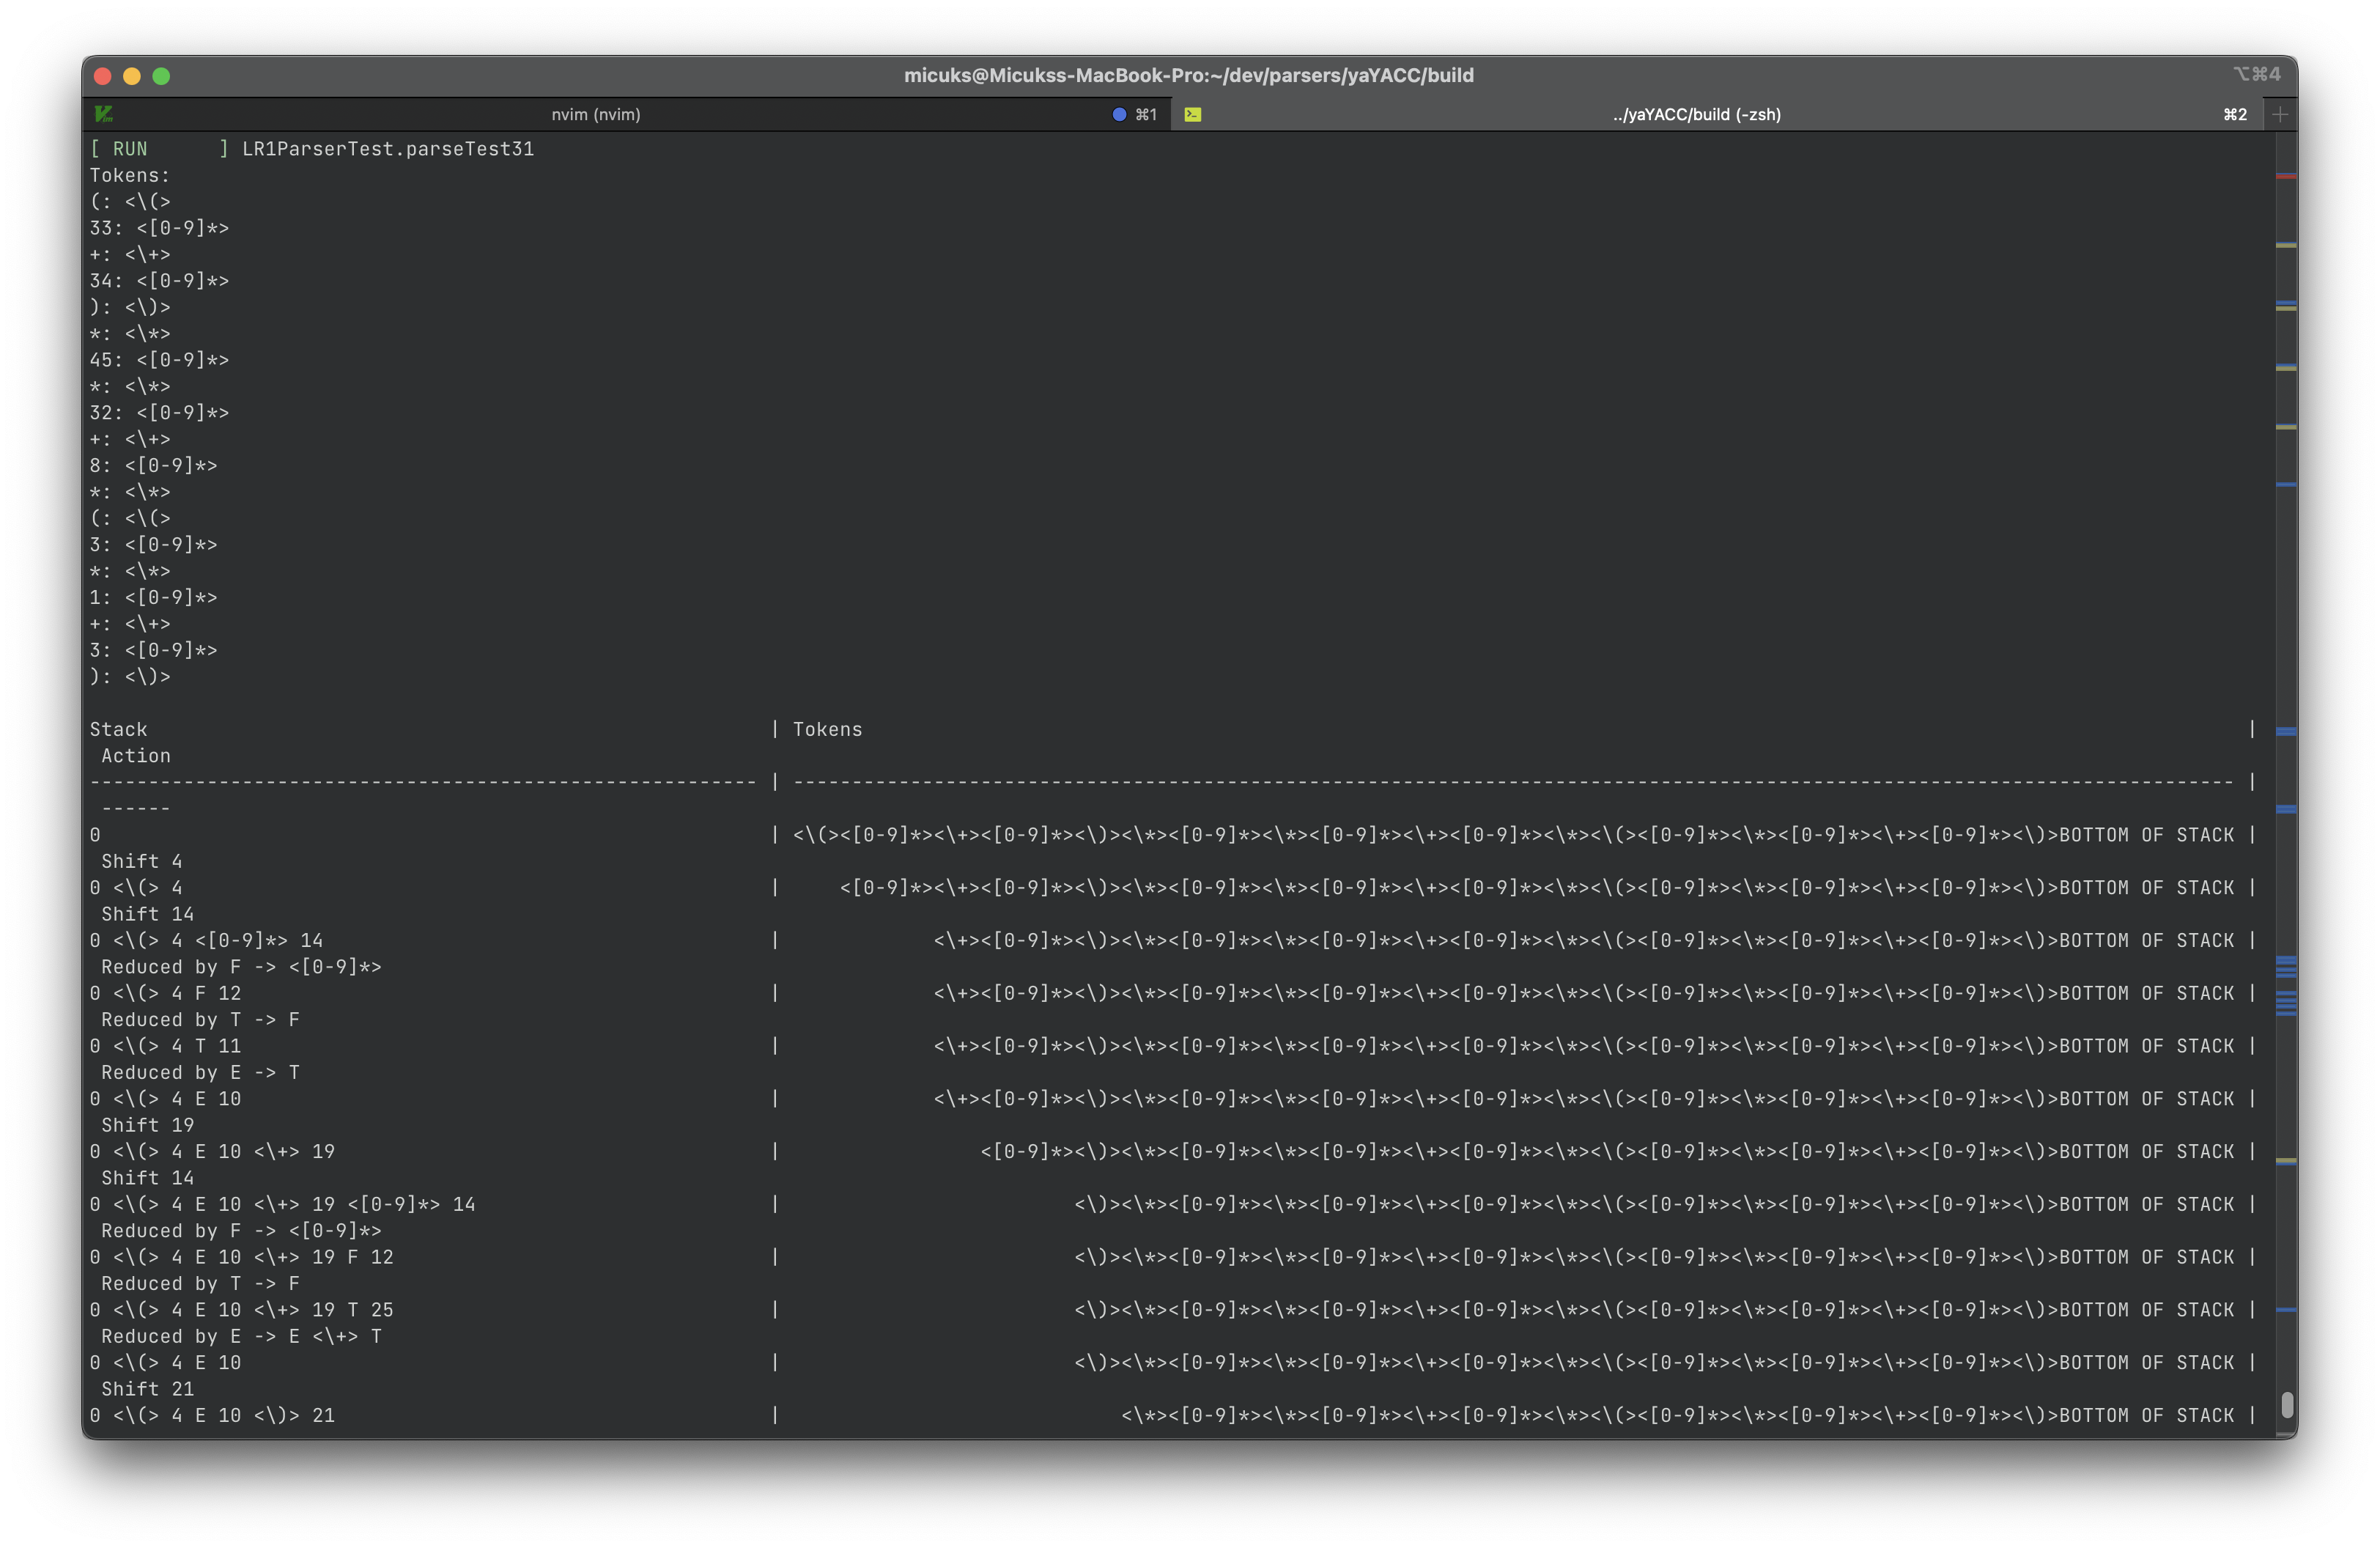
\includegraphics[width=0.95\textwidth]{figures/lr1复杂分析2.png}
	\end{center}
	\caption{复杂文法的LR1分析2}
	\label{fig:复杂文法的LR1分析2}
\end{figure}

对错误的输入能够正确拒绝, 如图\ref{fig:复杂文法的LR1分析3}.

\begin{figure}[ht!]
	\begin{center}
		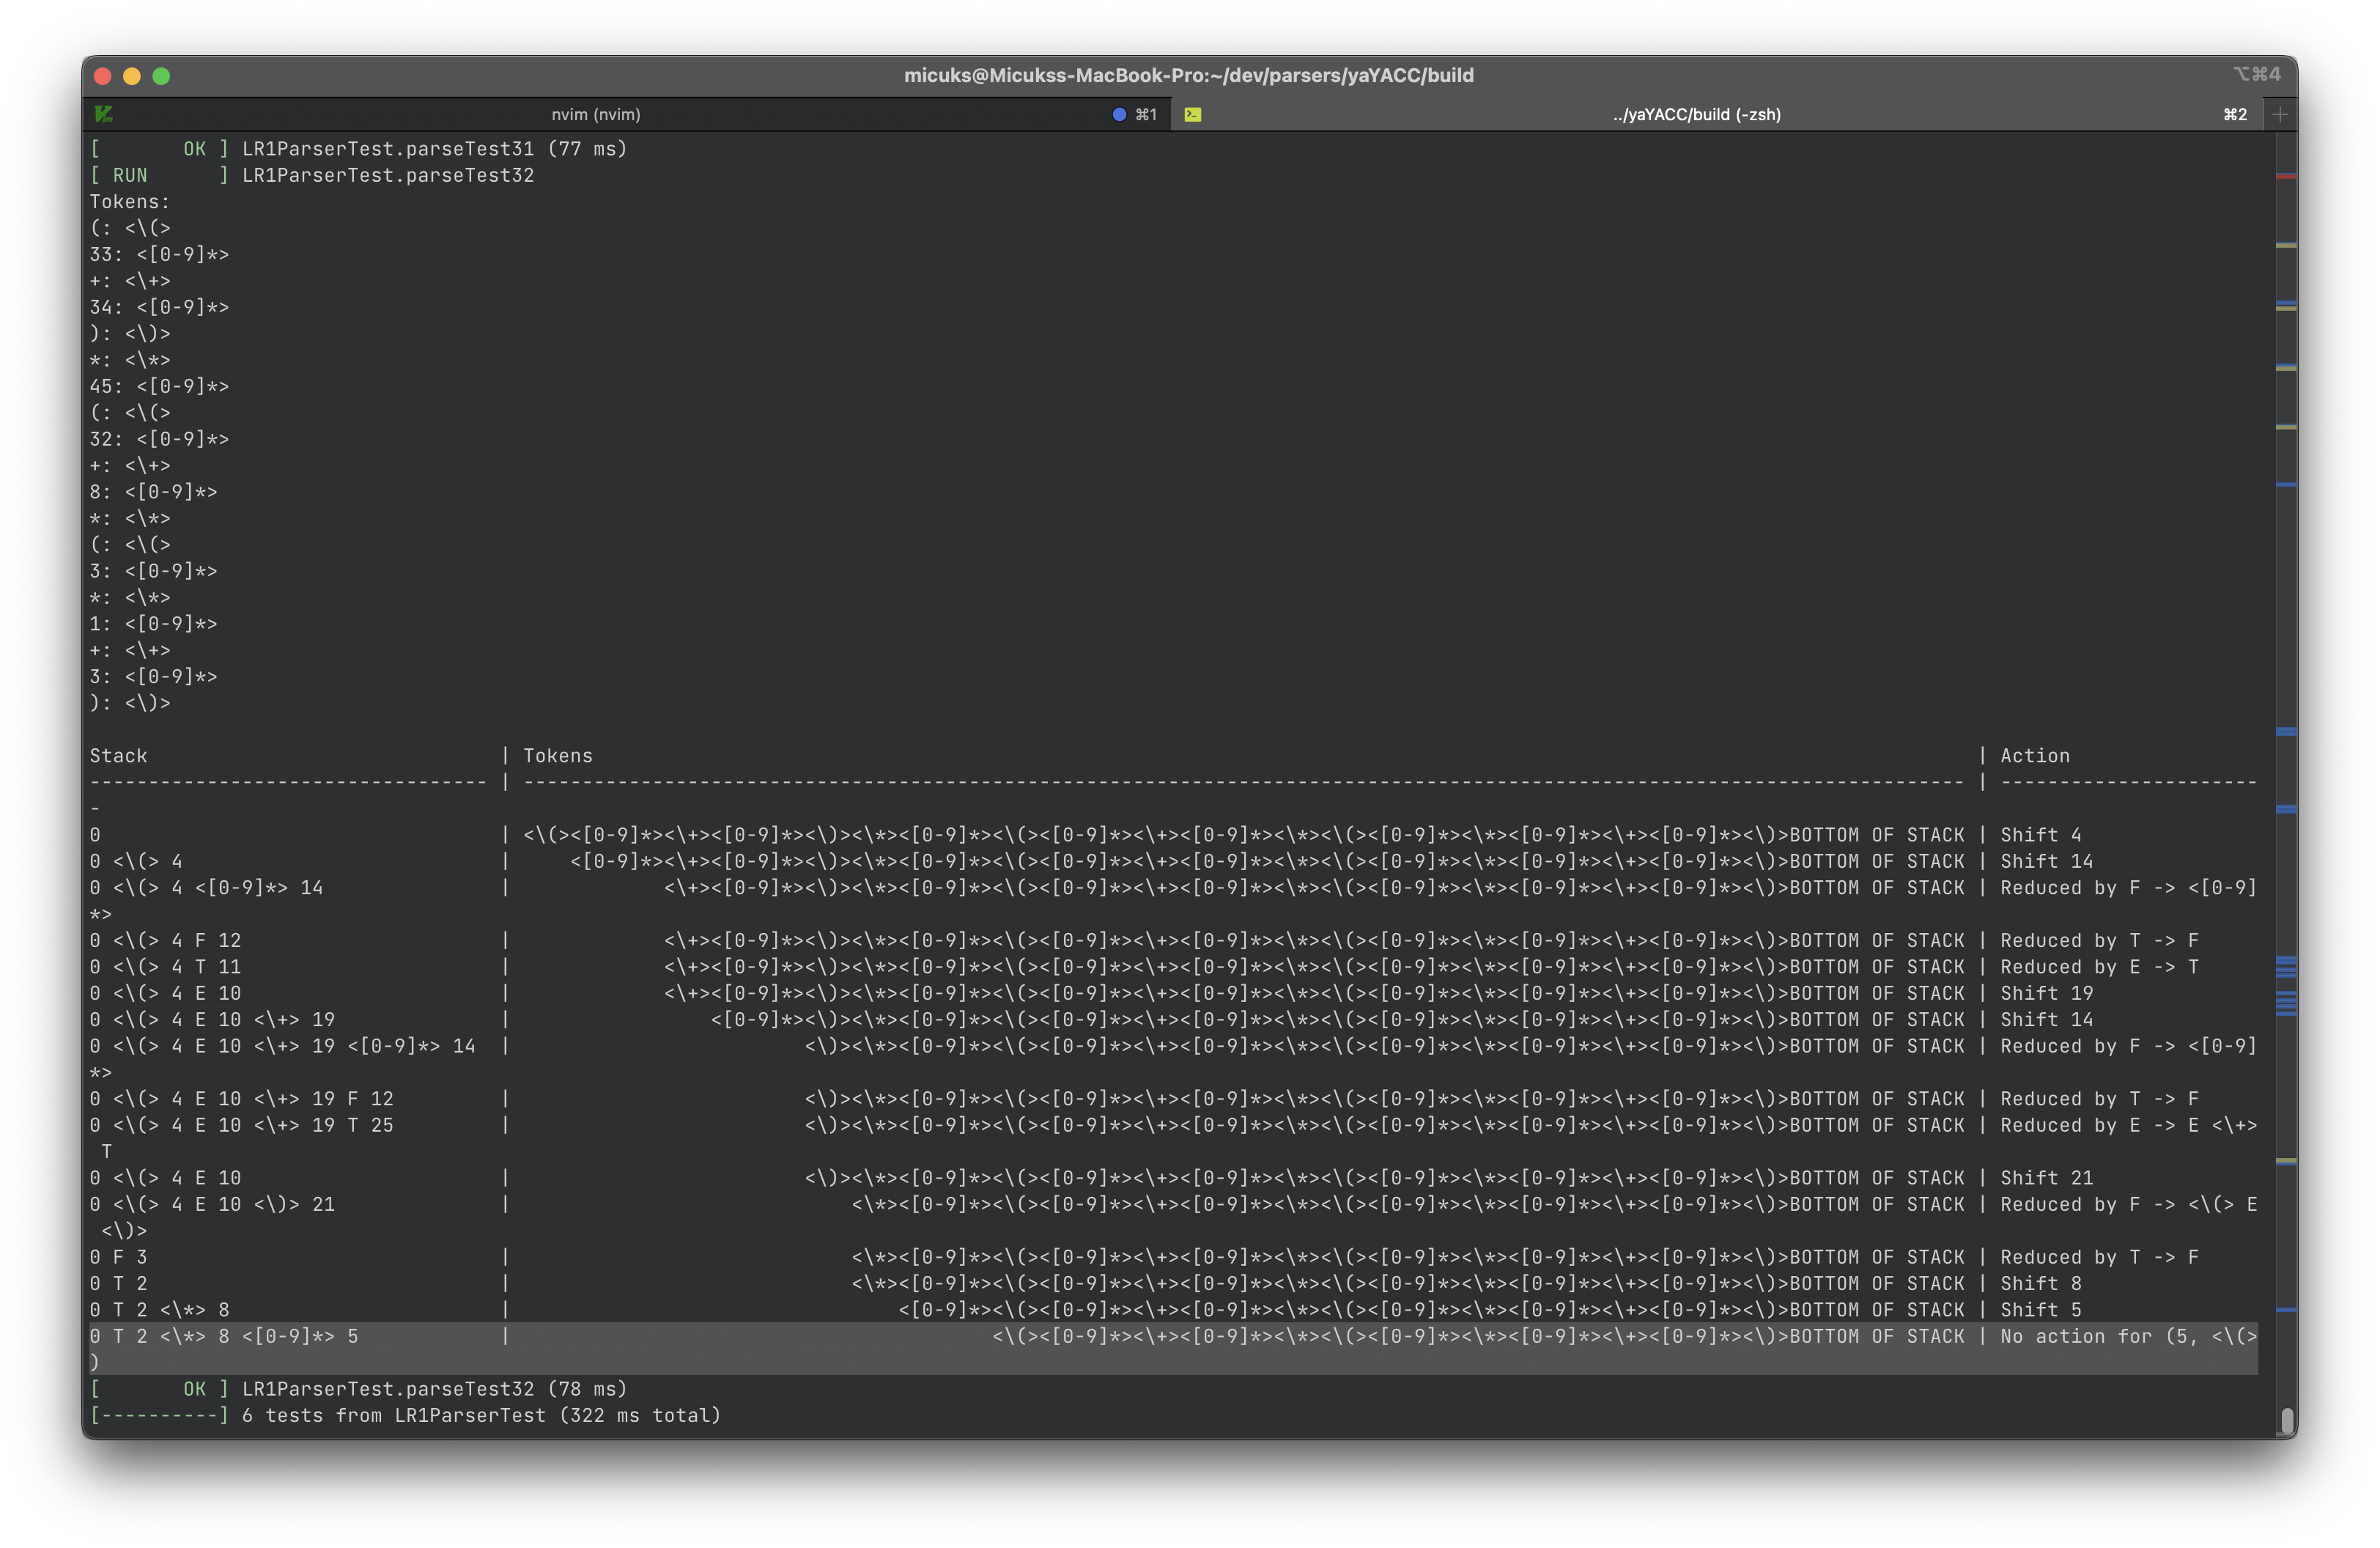
\includegraphics[width=0.95\textwidth]{figures/lr1复杂分析3.png}
	\end{center}
	\caption{复杂文法的LR1分析3}
	\label{fig:复杂文法的LR1分析3}
\end{figure}
